%#BIBTEX pbibtex Kitaev_kxy
%!TEX encoding = UTF-8 Unicode
\documentclass[reprint,amsmath,amssymb,aps,prx]{revtex4-2}
\usepackage[dvipdfmx]{graphicx}
\usepackage{dcolumn}
\usepackage{bm}
\usepackage{amsmath,amssymb}
\usepackage{color}
\newcommand{\red}[1]{\textcolor{red}{#1}}
\newcommand{\blue}[1]{\textcolor{blue}{#1}}
\newcommand{\magenta}[1]{\textcolor{magenta}{#1}}

\begin{document}

\title{Thermal Hall transport in extended Kitaev models}
\author{Tsuyoshi Okubo}
\affiliation{Institute for Physics of Intelligence, University of Tokyo, Tokyo, 113-0033, Japan}
\affiliation{JST, PRESTO, Saitama, 332-0012, Japan}
\author{Joji Nasu}
\affiliation{Department of Physics, Tohoku University, Sendai 980-8578, Japan}
\affiliation{JST, PRESTO, Saitama, 332-0012, Japan}
\author{Takahiro Misawa}
\affiliation{Beijing Academy of Quantum Information Sciences, Haidian District, Beijing 100193, China}
\affiliation{Institute for Solid State Physics, University of Tokyo, 5-1-5 Kashiwanoha, Kashiwa, Chiba 277-8581, Japan}
\author{Yukitoshi Motome}
\affiliation{Department of Applied Physics, University of Tokyo, Tokyo, 113-8656, Japan}

%}

\begin{abstract}
...
\end{abstract}

\maketitle
\section{Introduction}
Quantum Spin Liquid (QSL) is a highly correlated state of quantum spins 
without having any long-range orders. Among a variety of QSLs, Kitaev Spin Liquid (KSL) 
realized as the ground state of the honeycomb lattice Kitaev model \cite{Kitaev2006} 
is one of the most studied QSLs in two-dimensional spin models both by experiments and theories \cite{xxx}. 

Kitaev spin liquid is a キタエフスピン液体は大事。興味をもたれているというこをを書いた方がよい。保留。

Thermal Hall conductivity is one of the characteristic phenomena observed in the Kitaev spin liquid under applied magnetic field \cite{Kitaev2006}. Based on the Majorana fermions picture, the external magnetic field opens a gap in the bands of mobile Majorana fermions, and the chiral edge current appears. Due to the chiral edge current, the thermal Hall transport is induced. Because the chiral edge current is a current of majorana fermions, the thermal Hall conductivity takes the half-quantized value $\kappa_{xy}/T = 1/2 (\pi k_{\mathrm{B}}^2/(6\hbar))$ in the zero temperature limit.

Recently, a thermal Hall experiment for $\alpha$-$\mathrm{RuCl_3}$ claimed that the half-quantized thermal Hall conductivity was observed at finite temperatures \cite{RuCl_3_kxy}. Although $\alpha$-$\mathrm{RuCl_3}$ shows magnetic zigzag-order at zero field\cite{xxx}, the appearance of a non-magnetic state was discussed for intermediate magnetic field \cite{xxx}. The observed half-quantized thermal Hall conductivity indicates that stabilization of Kitaev spin liquid $\alpha$-$\mathrm{RuCl_3}$ under magnetic field. Similar half-quantized thermal Hall conductivities were also observed when we applied in-plane magnetic fields \cite{xxx}, and there are other reports consistent with Majorana fermion picture of KSL\cite{xxx,xxx}.

However, there remains controversy on interpreting the observed thermal Hall transport as the evidence of KSL. For example, the observed thermal Hall conductivity shows an overshoot of the half-quantized value for higher temperatures, and the origin of such overshooting behaviors has not been resolved. In addition, real compounds including $\alpha$-$\mathrm{RuCl_3}$, could contain additional interactions such as the Heisenberg interactions, and off-diagonal $\Gamma$ and $\Gamma'$ interactions \cite{...}. The effect of such additional interactions to the thermal Hall conductivity beyond the perturbation theories \cite{xxx} is alos not clear so far.

Furthermore, several later experiments for $\alpha$-$\mathrm{RuCl_3}$ discussed relationship to quantum oscillations observed in the longitudinal thermal conductivity\cite{xxx}, topological magnons\cite{xxx}, para-magnon\cite{xxx}, or phonon\cite{xxx}, and the origin of the thermal Hall conductivity has not been settled. To resolve the origin of the thermal conductivity observed in experiments, it is demanding to performed analysis based on Kitaev model without assuming any quasiparticle excitations.

Although the thermal Hall transport in the pure Kitaev model has been well understood in the limit of zero temperature and zero magnetic field\cite{Kitaev2006}, the discussion beyond the perturbation theory is limited. For finite temperature properties, we may use Monte Carlo simulation for zero magnetic field \cite{NasuUM2014,NasuUM2015}. Theses calculations successfully showed double-peak structure in specific heat and its relationship to the Majorana fermions. Unfortunately, however, in order to treat finite magnetic fields necessary for thermal Hall transport, we need to consider an effective interaction justified only for sufficiently small magnetic fields to avoid negative signs \cite{NasuYM2017}. Numerical simulations on the effective model showed non-monotonic temperature dependence of the thermal Hall conductivity:it has a weak peak at high temperature and converges to the half-quantized value \cite{NasuYM2017}. However, the peak value is much smaller than the half-quantized value, and then, the huge $\kappa_{xy}$ beyond the half-quantized value, such as the one observed in the experiment of $\alpha$-$\mathrm{RuCl_3}$, has not been explained by the effective model based on the perturbation theory.

\blue{\cite{Rau2014,Rau2014pre}はどこかで引用}

Similarly, the effect of the symmetric off-diagonal interactions, called $\Gamma$ and $\Gamma'$ terms, have been investigated based on the perturbative treatment justified in the situation of small magnetic fields and small off-diagonal interctions \cite{TakikawaF2020, YamadaF2021}. In the case of $\Gamma'$ interactions, it was shown that the $\Gamma'$ introduces an additional contribution proportional to both of $\Gamma'$ and the magnetic field in the gap of Majorana-fermion band \textcolor{red}{(Is it better to explicitly write down the relationship between the gap and parameters? If so, we may need to define the Hamiltonian before this paragraph.)}\cite{TakikawaF2020}. Thus the total gap is increased or decreased depending on the sign of the $\Gamma'$ interaction, and then the finite-temperature behaviors of the thermal Hall conductivity might largely depend on the sign of $\Gamma'$. Based on the similar perturbation theory, Ref.~\cite{YamadaF2021} discussed that the effect of the $\Gamma$ interaction appeared as the third order contribution. Although it indicates that the effect of $\Gamma$ in the thermal Hall transport is less than that of $\Gamma'$, the same analysis also showed a possible quantum phase transition induced by the effective interaction from the third order perturbation, and therefore, non-trivial effect might be possible from the phase transition due to $\Gamma$ interaction. Note that, as we mentioned, these analyses are based on the perturbation theory justified for small $\Gamma$ and $\Gamma'$. Furthermore, the connections to the thermal Hall transport was in the zero temperature limit. Thus, to understand effect of the off-diagonal interactions at finite temperatures, we need analysis beyond the perturbation theory.

As the origin of the thermal Hall transport at a finite temperature, we can also consider topological magnons excited from the magnetic order induced by the applied magnetic fields \cite{McClartyDGRPMP2018,Joshi2018}. The edge modes due to such topological magnons exist at high energies, and then the corresponding thermal Hall transport becomes zero in the zero temperature. However, at a finite temperatures, we need to consider a cotributions from such topological magnons in addition to the contributions from the Majorana fermions. In realistic situations, the thermal Hall transport might not be soley explained by the Majorana fermions or the topological magnons. To understand the thermal Hall transport at a finite temperature, we need to treat complicated mixture of these contributions. 

In this paper, we investigate the thermal Hall transport in Kitaev systems by numerical simulation based on tensor network, thermal pure quantum states, and classical approximations, beyond the perturbation theory. We properly define the energy current from the model Hamiltonian, and calculate edge current in the systems with open boundaries. This treatment does not assume any origins of the thermal Hall transport, and consider any contributions on equal footing.  We see that thus calculated thermal Hall conductivity shows clear overshooting behavior similar to the experimental observations, indicating that the experimentaly observed thermal Hall conductivity might be explained from simple models. We also discuss the effect of off-diagonal interactions to the thermal Hall conductivity. Indeed, we will see that depending on the sign and a type of the off-diagonal couplings, the thermal Hall conductivity can change its sign for finite temeperature. 

The remaining part of this paper is organized as follows....


\section{Model}
To investigate the thermal Hall transport in Kitaev systems, we consider an extended Kitaev model containing the off-diagonal $\Gamma$ and $\Gamma'$ interactions together with the Kitaev interaction on the honeycomb lattice (Fig.~\ref{fig:lattice}). The Hamiltonian of the model under a magnetic field is given as 
\begin{equation}
 \mathcal{H} = \sum_{\gamma = x,y,z} \sum_{\langle i,j \rangle_\gamma}\mathcal{H}_{ij}^\gamma -  \sum_{i,\gamma} h^\gamma S_i^\gamma,
 \label{eq:model-Hamiltonian}
\end{equation}
with
\begin{align}
 \mathcal{H}_{ij}^\gamma &= \Bigl[ K S_i^\gamma S_j^\gamma + \Gamma\left( S_i^\mu S_j^\nu + S_i^\nu S_j^\mu \right) \notag\\
&\qquad + \Gamma'\left( S_i^\mu S_j^\gamma + S_i^\nu S_j^\gamma + S_i^\gamma S_j^\mu + S_i^\gamma S_j^\nu \right) \Bigr]\\
&= \sum_{\alpha,\beta = x,y,z} J_{\alpha\beta}^\gamma S_i^\alpha S_j^\beta, 
\end{align}
where $\langle i,j\rangle_\gamma$ means the nearest neighbor pair on the $\gamma$-bond, and $(\mu, \nu, \gamma)$ is a permutation of $(x,y,z)$. Through out the paper, we consider the ferromagnetic Kitaev interaction $K= -1$. \red{We also set the amplitude of the primitive translation vector of the honeycomb lattice to the unit length and $k_B = 1$.} We discuss, typically, physical quantities for the model on \red{$(L, L') = (6, 6)$}shown in Fig.~\ref{fig:lattice}(a). In the Appendix \ref{sec:XTRG_Bench}, we compare the results with those of \red{$(L, L') = (4, 8)$}. 

\blue{XC4、XC6という表現が少しマニアックな気がします。$(L,L')=(4,6),(6,6)$とかの方がわかりやすい?
もしくは、$L_X=2L$、$L_Y=L'/2$のように基本並進ベクトル基準にして、実空間を$\bm{R}=(X,Y)$で表現した方がよいかもしれないです。
この場合、site positionも$\bm{R}_i$として、$\kappa_{XY}$のように表現すべきかもしれません。}\red{$(L,L')$方式を採用してみる。}

\begin{figure}
  \begin{center}
    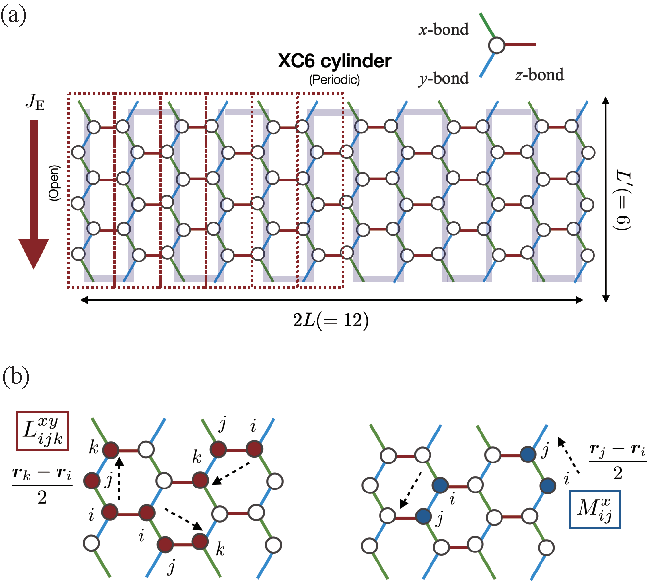
\includegraphics[width=\linewidth]{Figs/lattice.pdf}
  \end{center}
  \caption{(a) Schematic view of \red{an $(L, L') = (6, 6) $ honeycomb lattice consisting of 72 sites}. Along the vertical direction, we impose the periodic boundary condition, while the left and the right boundaries are open. We consider the thermal current $J_{\mathrm{E}}$ in a downward direction indicated by the arrow. In the tensor network simulation, we consider a snake like matrix product operators indicated by the gray thick line behind the lattice. (b) Graphical representations of the three-body ($L$) and the two-body ($M$) terms in the definition of the thermal current \eqref{eq:def_J}.}
  \label{fig:lattice}
\end{figure}

\red{To investigate the magnetic property of the model, we defined the magnetization parallel to the appliged magnetic field, $M_{\parallel}$, as $M_\parallel=\vec{M}\cdot\vec{h}/|\vec{h}|$, where $\vec{M} = \frac{1}{N}\sum_i \vec{S}_i$ is the total magnetization.}

The ground state phase diagram of this extended Kitaev model have been investigated by xxx (the zigzag state is stabilized for small $\Gamma$ and $\Gamma'$.... Thus, this model might be suitable to investigate the relevant effect of off-diagonal interaction to the thermal Hall conductivity in real compounds including $\alpha$-$\mathrm{RuCl_3}$.


\section{Method}
In this section, we discuss how to define the thermal Hall conductivity for finite size clusters described above. Then, we explains three numerical methods for calculating finite temperature properties of the model. To investigate quantum spin models, we employ two types of methods. For smaller clusters we use the thermal pure quantum state (TPQ) method, while we employ a tensor network based method for larger clusters. As a reference to the quantum model, we also investigate classical spin model with the same interaction coefficients calculated by Monte Carlo simulations.

  \subsection{Thermal Hall conductivity}
  To investigate the thermal Hall conductivity in the Kitaev systems, we firstly define the energy current through the commutation relation between the Hamiltonian and the energy porlalization, $\bm{P}_{\mathrm{E}}$, as $\bm{J}_{\mathrm{E}} =  i \left[\mathcal{H}, \bm{P}_{\mathrm{E}}\right] \notag$\blue{, where the reduced Planck constant is set to be unity [$k_B$を1にすることと長さの単位についても言及した方がよいかもしれません。]}\red{Modelのところの$K=-1$のところに単位などについて、まとめて書くことにした。$\hbar$はとりあえずここのまま。}. The energy porlization is defined as 
\begin{equation}
 \bm{P}_{\mathrm{E}} = \sum_{\alpha,\beta,\gamma}\sum_{\langle i,j\rangle_\gamma} \frac{\bm{r}_i + \bm{r}_j}{2} J_{\alpha\beta}^\gamma S_i^\alpha S_j^\beta - \sum_{i,\gamma} \bm{r}_i h^\gamma S_i^\gamma,
\end{equation}
where $\bm{r}_i$ is the position of the site $i$. By substituting $\bm{P}$ into the definition of $\bm{J}_{\mathrm{E}}$, we obtain
  \begin{align}
   \bm{J}_{\mathrm{E}} &=  i \left[\mathcal{H}, \bm{P}_{\mathrm{E}}\right] \notag \\
&= \sum_{\gamma,\gamma'}\sum_{\langle i,j,k\rangle_{\gamma,\gamma'}} \frac{\bm{r}_k-\bm{r}_i}{2}L_{ijk}^{\gamma\gamma'} + \sum_{\gamma}\sum_{\langle i,j\rangle_{\gamma}} \frac{\bm{r}_j-\bm{r}_i}{2}M_{ij}^{\gamma} 
   \label{eq:def_J},
  \end{align}
where $L_{ijk}^{\gamma\gamma'}$ is the cotribution from three-spin correlations,
\begin{equation}
 L_{ijk}^{\gamma\gamma'} = \sum_{\alpha,\beta,\alpha',\beta',\gamma''} J_{\alpha\beta}^\gamma J_{\alpha'\beta'}^{\gamma'} \epsilon_{\alpha\gamma''\alpha'} S_i^\beta S_j^{\gamma''}S_k^{\beta'},
\end{equation}
and $M_{ij}^\gamma$ represents the contribution from two-spin correlations,
\begin{equation}
 M_{ij}^{\gamma} = \sum_{\alpha,\beta,\gamma',\gamma''} J_{\alpha\beta}^\gamma h_{\gamma'} \epsilon_{\gamma'\alpha\gamma''} \left(S_i^{\gamma''} S_j^{\beta} - S_i^{\beta} S_j^{\gamma''} \right).
\end{equation}
Note that $\epsilon_{\alpha\beta\gamma}$ means the completely antisymmetric tensor come from the commutation relation between spins. 

 As shown in Fig.~\ref{fig:lattice} (a), we consider the energy current along vertical direction of the cluster (circumferential direction of the cylinder), and define it as $J_{\mathrm{E}}$ \blue{[絶対値に見えてしまうので、$J_{\mathrm{E}}^\parallel$など文字を変えた方がよい?]}\red{(仰る通りだと思いました。$J_{\mathrm{E}}^\parallel$を採用します。)}. Note that due to the symmetry of the system, $J_{\mathrm{E}}$ is exactly equal to zero for any temperatures. To pick up contribution to the Hall current from $J_{\mathrm{E}}$, we consider that each term in Eq.\eqref{eq:def_J} represents the current density at $(\bm{r}_i + \bm{r}_j)/2$ and sum them up from the left edge to the center of the system. We also define the current at each line as the sum within a box indicated in Fig.~\ref{fig:lattice}(a). To avoid unnecessary boundary effect from the definition of boxes, we move the right edge of the box slightly to the right so that $L^{xy}_{ijk}$s corresponding to the diagonal directions of each hexagon are in the same line.
\blue{[この定義の部分は要修正ですよね?。lineのナンバリングとboxとの関係が必要。$l$番目のlineに含まれる局所熱流の図があった方がよいと思います。zigzag chainを中心としたboxにして、box内部と右端のedgeと交差する線分で定義された局所熱流を含む、など明示した方がよいと思います。
The local energy current $L_{ijk}^{\gamma\gamma'}$ ($M_{ij}^{\gamma}$) is defined on the line segment connecting sites $i$ and $k$ ($i$ and $j$).
Here, we introduce the energy current $J_{{\rm E},l}^\parallel$ along the zigzag chain labelled by line $l$ such that $J_{{\rm E},l}^\parallel$ includes the contributions from the local currents on the segments inside the box surrounding the chain and across its right edge, which are shown in Fig.***. 
とかでしょうか。このあと、thermal currentとして$J_{\rm E}^\parallel=\sum_{l=1}^{L/2??}J_{{\rm E},l}^\parallel$とした方がよいかも。
]}

By taking the derivative of $J_{\mathrm{E}}$ with respected to the temperature, we obtain the thermal Hall conductivity as 
\begin{equation}
 \kappa_{xy} \equiv \frac{2}{L'} \frac{d \langle J_{\mathrm{E}}\rangle_{T}}{d T},
\label{eq:def_kxy}
\end{equation}
where $\langle J_{\mathrm{E}} \rangle_T$ represents the thermal average at a temperature $T$, and $L'$ is the length along the circumferential direction of the cylinder (Fig.~\ref{fig:lattice}(a)). \textcolor{red}{(Should I mention the details of numerical derivatives here?)}\textcolor{red}{(We may change the definition of $L'$. It affects the figures of classical simualations.)}

\blue{($L$は倍で$L'$が半分なのが基本並進ベクトルに沿った定義でしょうか。Fig.~\ref{fig:lattice}(a)が$12\times 3$に対応?)}

  \subsection{Tensor network method}
  In this section, we explain the tensor network method used in our study for larger clusters which cannot be treated by the thermal pure quantum state method. To investigate finite temperature properties of the model, we approximate a density matrix of the system at a inverse temperature $\beta$, $\rho(\beta) = e^{-\beta\mathcal{H}}$, as an matrix product operator (MPO) with the bond dimension $D$ (See Fig.~\ref{fig:XTRG}(a)). The string of the MPO is arranged in a snake form as shown in the gray line in Fig.~\ref{fig:lattice} (a). 

  To optimize the tensors in an MPO as the density matrix at $\beta$, we employ the exponential thermal tensor renormalization group (XTRG) approach \cite{Chen2018,Li2020}, which has successfully calculate finite temperature properties of the Kitaev model \cite{Li2020}. In XTRG algorithm, we calculate the density matrix at $\beta$ through the relationship
\begin{equation}
 \rho(\beta)=\rho(\beta/2)\rho(\beta/2).
\end{equation}
When $\rho(\beta/2)$ is represented by MPO with the bond dimension $D$, $\rho(\beta)$ becomes an MPO with the bond dimension $2D$. We approximate this $\rho(\beta)$ by MPO with $D$ through the standard optimization procedure for the matrix product states (MPS) \cite{Chen2018}  (See Fig.~\ref{fig:XTRG}(b)). In particular, we employ the two-site update, and the computation cost of the XTRG algorithm scales as $O(D^4)$. As the initial condition of the XTRG algorithm, we prepare $\rho(\beta_0)$ with $\beta_0 = 10^{-7}$ through the approximated form $\rho(\beta_0) \simeq 1 - \beta_0\mathcal{H}$, where the Hamiltonian is represented as an MPO. We calculate the expectation value of an operator $\hat{O}$ through thus obtained $\rho(\beta)$ as $\langle \hat{O} \rangle = \mathrm{Tr}~\hat{O}\rho /\mathrm{Tr}~\rho$ (Note that our density matrix is not normalized). \red{The temperature derivative of $\langle \hat{O} \rangle$ is computed through numerical difference \cite{Chen2018}.}

In the followings, we mainly show the data with $D=500$ for $(L, L') = (6, 6)$ cylinder. Several benchmark calculations for different $D$s and a different lattice shape will be discussed in Apeendix~\ref{sec:XTRG_Bench}. 

\begin{figure}
  \begin{center}
    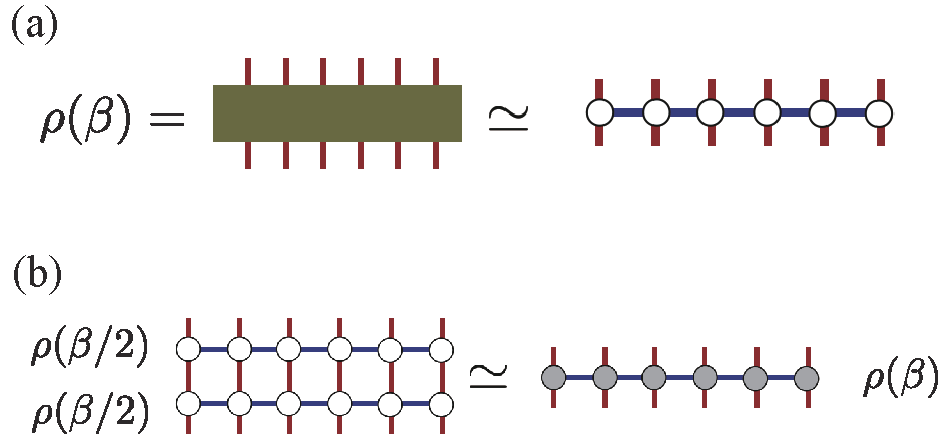
\includegraphics[width=\linewidth]{Figs/XTRG_MPO.pdf}
  \end{center}
  \caption{Tensor network diagram for the density operator approximation. (a) The density matrix is approximated as a matrix product operator with bond dimension $D$. Here, the horizontal line corresponds to the gray line in Fig.~\ref{fig:lattice}(a). (b) The density matrix at $\beta$ is calculated as $\rho(\beta)=\rho(\beta/2)\rho(\beta/2)$. The bond dimension of the obtained $\rho(\beta)$ is truncated to $D$ through the standard optimization procedure of MPS.}
  \label{fig:XTRG}
\end{figure}

  \subsection{Thermal pure quantum state}
In this section, we explain the basics of the canonical thermal quantum pure (cTPQ) state method~\cite{Sugiura_PRL2013}, 
\magenta{which enables us to calculate the finite temperature properties of quantum many-body systems using the power method. 
We note that several similar methods were independently proposed~\cite{Imada_JPSJ1986,Jaklic_PRB1994,Hams_PRE2000,Lloyd} before the proposal of the cTPQ method~[\onlinecite{Sugiura_PRL2013}].}
We construct the 
cTPQ state $|\Phi_{\rm cTPQ}^{p}\rangle$ as follows:
\begin{align}
|\Phi_{\rm cTPQ}^{p}(\beta)\rangle = \exp\Big[-\frac{\beta}{2}\mathcal{H}\Big]|\Phi_{\rm rand}^{p}\rangle,
\end{align}
where $\beta$ is inverse temperature and 
$|\Phi_{\rm rand}^{p}\rangle$ is the $p$th initial random vector, which uniformly distributed
on the $N_{\rm H}$ dimensional super sphere ($N_{\rm H}$ is the dimension of the Hilbert space of the given system).
Any local physical quantities at inverse temperature $\beta$
can be calculated as the expectation values of $|\Phi_{\rm cTPQ}^{p}(\beta)\rangle$, i.e.,
\begin{align}
\langle A(\beta)\rangle
=\frac{\langle \Phi_{\rm cTPQ}^{p}(\beta)|A|\Phi_{\rm cTPQ}^{p}(\beta)\rangle}
{\langle \Phi_{\rm cTPQ}^{p}(\beta)|\Phi_{\rm cTPQ}^{p}(\beta)\rangle}.
\end{align}
In the actual calculations, we calculate the 
cTPQ state as follows:
\begin{align}
&\exp\Big[-\frac{\beta}{2}\mathcal{H}\Big]|\Phi_{\rm rand}^{p}\rangle=U(\Delta\tau)^{k}|\Phi_{\rm rand}^{p}\rangle,\\
&U(\Delta\tau)=\exp\Big[-\frac{\Delta\tau}{2}\mathcal{H}\Big]\sim\sum_{n=0}^{n_{\rm max}}\frac{1}{n!}(-\frac{\Delta\tau}{2}\mathcal{H})^{n},\\
&\beta=k\Delta\tau,
\end{align}
where we take $n_{\rm max}=6$ and $\Delta\tau =0.02$.
We confirm that $n_{\rm max}=6$ ($\Delta\tau=0.02$) is sufficiently
large (small) for obtaining converged physical quantities 
in the calculated temperature region.

The cTPQ method gives the numerically exact
results within the statistical fluctuations,
which is defined by the statistical distribution of the initial random vectors.
To evaluate the fluctuations, i.e., the errors of the cTPQ method, 
we employ the bootstrap method.
Using the bootstrap method,
we evaluate the average values and 
error bars of physical quantities as follows.
\begin{enumerate}
\item Preparing $N_{\rm tot}$ random initial states and generating the cTPQ states.
\item Randomly choosing $P$ samples among $N_{\rm tot}$ cTPQ states allowing duplications. 
Repeating this procedure $M$ times and the mean value of the physical quantities $A$ 
at $m$th times is given by 
\begin{align}
A_{m}(\beta) = \frac{\sum_{p=1}^{P}\langle \Phi_{\rm cTPQ}^{p}(\beta)|A|\Phi_{\rm cTPQ}^{p}(\beta)\rangle}{\sum_{p=1}^{P}\langle \Phi_{\rm cTPQ}^{p}(\beta)|\Phi_{\rm cTPQ}^{p}(\beta)\rangle},
\end{align}
where $\langle A(\beta)\rangle_{p}$ is the physical quantities calculated by the cTPQ state 
which is generated by $p$th initial states.
\item From $A_{m}(\beta)$, the 
average value $\bar{A}(\beta)$
and the standard deviations (error bars, $\sigma[A(\beta)]$ ) are 
evaluated as
\begin{align}
&\bar{A}(\beta) = \frac{1}{M}\sum_{m=1}^{M}A_{m}(\beta), \\
&\sigma[A(\beta)] = \Big[\frac{1}{M-1}(\sum_{m=1}^{M}A_{m}(\beta)^2-\bar{A}(\beta)^2)\Big]^{1/2}.
\end{align}
\end{enumerate}

  \subsection{Classical Monte Carlo simulation}
Finally, we show the details of the classical Monte Carlo simulations.
In this method, an $S=1/2$ spin at each site is regarded as a classical vector.
Namely, a classical spin at site $i$ is parameterized by $\theta_i$ and $\phi_i$ as
$\bm{S}_i = \frac{1}{2}(\sin\theta_i\cos\phi_i, \sin\theta_i\sin\phi_i, \cos\theta_i)$.
In the calculation of the thermal average, the integral $\int \prod_i d\phi_i d\theta_i \sin\theta_i$ is evaluated by using the Markov-chain Monte Carlo method.
To accelerate the computation speed and avoid trapping the spin configuration at local minimums, we use the replica exchange method \cite{Hukushima1996}.
In the simulations, we prepare 48~replicas with different temperatures.
We perform 10~000~000~MC steps for measurement after 10~000~MC steps for thermalization in the 800-site cluster with $L=10$ and $L'=40$ (see Fig.~\ref{fig:lattice}(a)).
\blue{The temperature derivative of $\langle O \rangle$ is evaluated by the correlation with ${\cal H}$ as  $d\langle O \rangle/dT=\left(\langle A{\cal H}\rangle -\langle A\rangle \langle {\cal H}\rangle \right)/T^2$, while it is computed as a numerical difference in the case of the quantum system.
[要確認]\red{(この記述通りで、数値微分でOK。量子系のところにちゃんと説明を書く。$\to$書いた。)}
}


\section{Result}
  \subsection{Pure Kitaev model}
   %\subsubsection{Ferromagnetic case}
   \subsubsection{\red{magnetic filed along [111] direction}}
Firstly, we discuss the case where ferromagnetic Kitaev model is under a magnetic field parallel to $[111]$ direction. In this set up, we expect positive $\kappa_{xy}$ for small magnetic fields $h = |\vec{h}|$ in the zero temperature limit \cite{Kitaev2006}. 

Fig.~\ref{fig:CMF_pure}(a) shows the temperature dependence of the specific heat for various magnetic fields. We see clear double peak structure for each magnetic field which is considered to be a characteristic of the separation of energy scales of localized and mobile Majorana fermions \cite{NasuUM2014,NasuUM2015}. The low-temperature peaks move to higher temperature as we increase the magnetic field, while the high-temperature peaks are almost independent on the magnetic field. Although the slight non-smooth temperature dependencies for $h \lesssim 0.03$ is considered due to the small $D$ effect, the specific heats for $h \gtrsim 0.04$ is smooth and the present $D=500$ seems to be sufficient for discussing thermal properties of the model. Additional discussions on the bond-dimension dependencies are in App.~\ref{sec:XTRG_Bench}.

\begin{figure}
  \begin{center}
    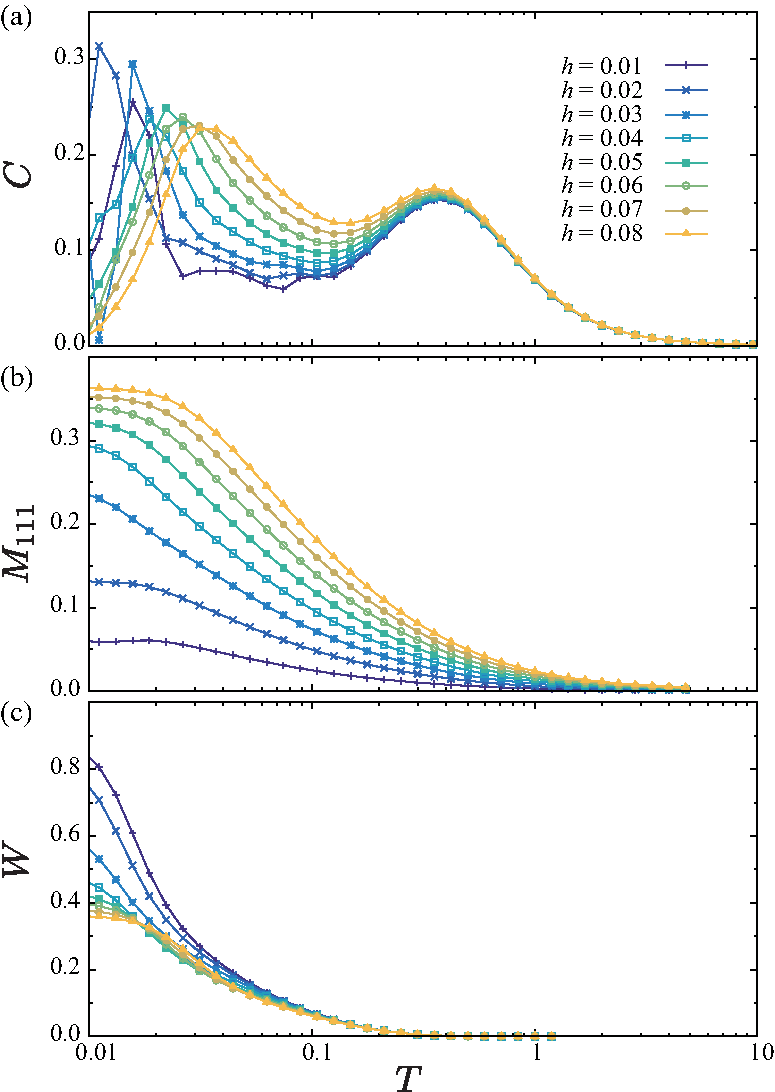
\includegraphics[width=0.9\linewidth]{Figs/plot_CMF.pdf}
  \end{center}
  \caption{\textcolor{red}{(To be updated)}Temperature dependence of (a) the specific heat (b) the magnetic moment, and (c) the flux of the ferromagnetic Kitaev model for various external magnetic field parallel to $[111]$ direction.}
  \label{fig:CMF_pure}
\end{figure}

\blue{[magnetizationの定義が必要かと思います。$M_{111}$より、$\bm{M}=\frac{1}{N}\sum_i \bm{S}_i$として、$M_\parallel$を$M_\parallel=\bm{M}\cdot\bm{h}/|\bm{h}|$と定義した方がよいかもしれません。]}\red{この提案を採用します。}

For such $h \gtrsim 0.04$ at low temperature, the magnetizations are slightly high as $M_{111} \ge 0.3$ (Fig.~\ref{fig:CMF_pure}(b)), and also the fluxes are $W \ge 0.4$ (Fig.~\ref{fig:CMF_pure}(c)), which is smaller than $W=1$ expected for the zero magnetic filed. Note that there is a phase transition between the chiral spin liquid and the para magnetic phases around $h_c \simeq 0.02$ \cite{ZhuKSF2018,LeeKCOYKK2020}. However in the present calculations we do not observe clear singularity corresponding to the phase transition, probably due to a finite size effect. 

In Fig.~\ref{fig:J_line}, we show the energy current of the model for two representative magnetic fields, $h=0.04$ and $h=0.08$. We see that the energy currents are almost zero in the high temperature limit, and they become negative in low temperatures. This behavior indicates that $\kappa_{xy} \propto d J_{\mathrm{E}}/d T$ is positive and consistent with the expectation in the zero temperature limit. 
\begin{figure*}
  \begin{center}
    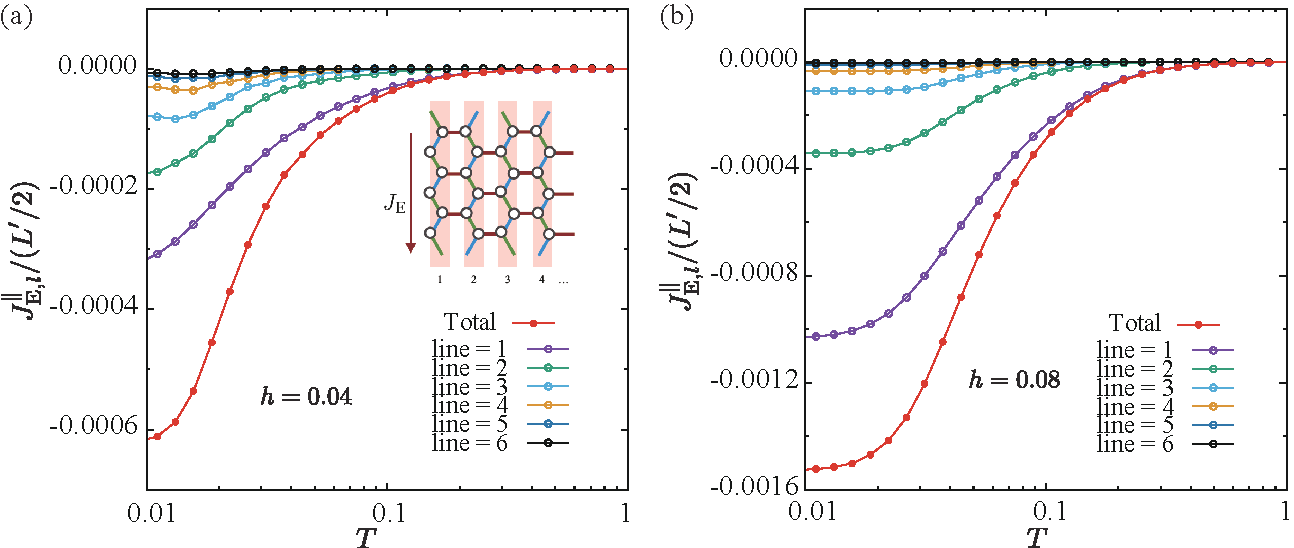
\includegraphics[width=0.9\linewidth]{Figs/J_line_all.pdf}
  \end{center}
  \caption{\textcolor{red}{(Need to check the definition of $L_y$.)}Temperature dependence of the energy current of the ferromagnetic Kitaev model under (a) $h=0.04$ and (b) $h=0.08$. In addition to the total energy current, contribution from each line is presented.}
  \label{fig:J_line}
\end{figure*}

We also plot the position dependent energy currents in Fig.~\ref{fig:J_line}. When we go from the edge side (line = $1$) to the center (line = $6$), the amplitude of the currents decreases. Because the contributions from the center region are sufficiently small, we consider that the our total energy current $J_{\mathrm{E}}$, which is the sum of contributions from all lines up to centers, correctly captures the edge current. We also realize that the decay of the current amplitude toward the center becomes faster when we increase the magnetic field. This behavior might be explained by the increase of the excitation gap of quasi particles carrying the energies. 


By taking the numerical derivative of $J_{\mathrm{E}}$, we obtained the thermal Hall conductivity as Eq.~\ref{eq:def_kxy}. Thus obtained $\kappa_{xy}/T$s are shown in Fig.~\ref{fig:k_all_pure}(a). Except for small magnetic fields, we see clear peak structure in Fig.~\ref{fig:k_all_pure}. The peak temperatures move to higher temperature as we increase $h$, they seem to be correlated with the low-temperature peaks of the specific heat. Interestingly, $\kappa_{xy}/T$ becomes much larger than the half-quantized value for intermediate temperatures. Such an overshooting behavior was not observed in the previous numerical calculations on an effective model with perturbative treatment of the magnetic fields \cite{NasuYM2017}. Note that in the low temperature limit, the calculated $k_xy/T$ does not converge to the half-quantized value. Due to the finiteness of the circumferential directions, even for the sufficiently small $h$, the expected chiral edge mode has a finite gap, and then $k_xy/T$ becomes zero in the low temperature limit. Thus, in the present calculations, we do not deeply discuss behaviors of $k_xy/T$s for lower temperatures. 

In Figs.~\ref{fig:k_all_pure}(b) and (c), we plot the contributions from the three-body and the two-body correlations, respectively, to the total $\kappa_{xy}/T$. We see that the three-body correlations are the dominant contributions to $\kappa_{xy}/T$ for all magnetic fields. Although the two-body correlations are less dominant, quantitatively, we also see peak structure in them for $h \ge 0.04$.

\begin{figure}
  \begin{center}
    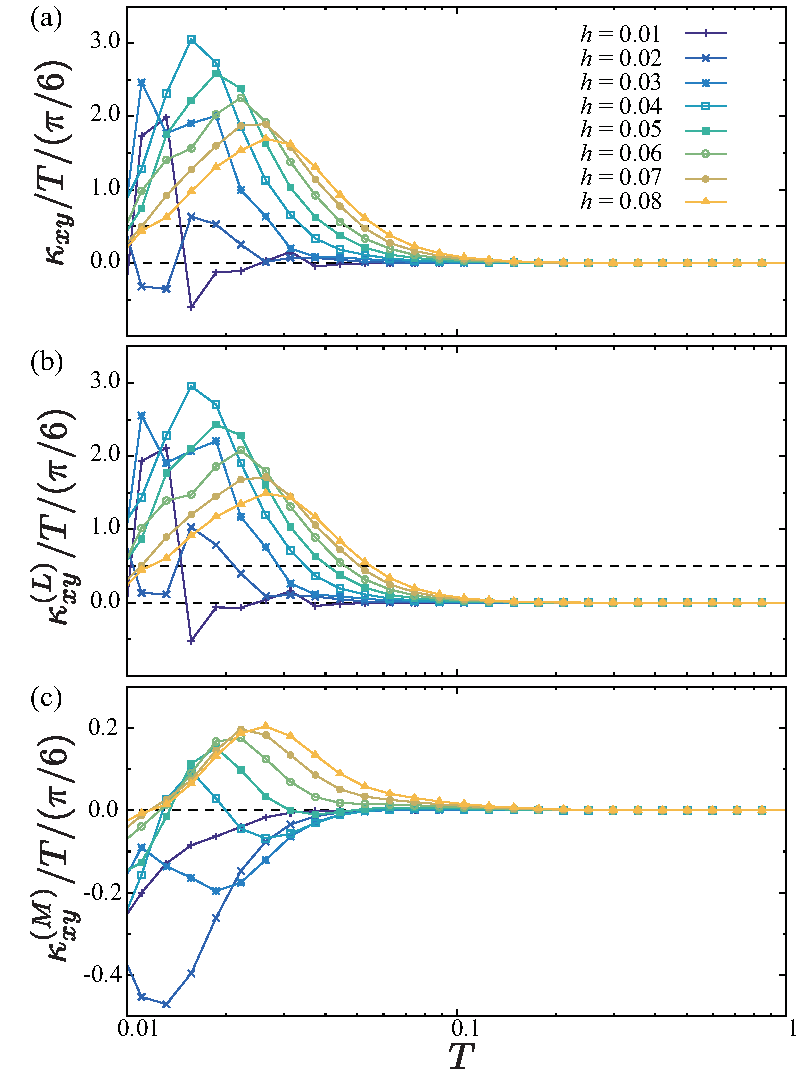
\includegraphics[width=0.9\linewidth]{Figs/plot_k_all.pdf}
  \end{center}
  \caption{\textcolor{red}{(To be updated)}(a) Temperature dependence of $\kappa_{xy}/T$ of the ferromagnetic Kitaev model for various magnetic fields parallel to $[111]$ direction. Two horizontal dashed lines indicate $\kappa_{xy}/T = 0$ and the half-quantized value. (b,c) Contributions from the three-body ($L$) and and the two-body ($M$) terms, respectively.}
  \label{fig:k_all_pure}
\end{figure}


   \subsubsection{Field angle dependence}
Next, we see the field-angle dependence in $\kappa_{xy}/T$. Here we pick up two representative magnetic fields, $h=0.04$ and $h=0.08$, and consider three directions of magnetic fields as $\vec{h} \parallel [111]$, $[11\bar{2}]$, and $[\bar{1}10]$. 

Figs.~\ref{fig:k_all_h0.04_ab} and \ref{fig:k_all_h0.08_ab} shows temperature dependencies of $\kappa_{xy}/T$ for three magnetic-field directions at $h = 0.04$ and $h=0.08$, respectively. We see that the change of the field direction from $\vec{h} \parallel [111]$ to  $\vec{h}\parallel [11\bar{2}]$, $\kappa_{xy}/T$ changes the sign of $\kappa_{ky}$ to negative. Such sign change can be seen also in the contributions from the three-body correlations, while we do not find clear corresponding behavior in the contributions from the two-body correlations. In particular, in the case of $h = 0.08$, both of $\kappa^{(M)}_{xy}/T$s show positive peaks for $\vec{h} \parallel [111]$ and $\vec{h} \parallel [11\bar{2}]$. Note that, in the case of $\vec{h} \parallel [\bar{1}10]$, $\kappa_{xy}/T$ is equal to zero\blue{.
This is understood from the fact that the Hamiltonian is invariant under the following two operations simultaneously:
The $C_2$ rotation along the $[\bar{1}10]$ axis in the spin space transferring $(S^x,S^y,S^z)$ to $(-S^y,-S^x,-S^z)$ and the rotation of the honeycomb plane along the $z$~bond in the real space, which exchanges the $x$ and $y$~bonds.
However, the rotation of the honeycomb plane inverts the component of the position vector $\bm{r}$ along the zigzag edge, and thereby, the thermal current along the zigzag edge should be zero.
Note that the above argument is applicable in the presence of the $\Gamma$ and $\Gamma'$ interactions.
}
% , which is expected by the symmetry. \textcolor{red}{(Probably, it it better to move Nasu-san's discussion in classical MC section here.)} 
The change of $\kappa_{xy}$ depending of the field angles is probably explained both by the Majorana fermions \cite{Kitaev2006} and the topological magnons \cite{ChernZK2021}. Although the sign of $\kappa_{xy}$ in the case of topological magnon is different from our calculations, in principle, it is difficult to separate two contributions in thermal Hall conductivity at a finite temperature.

\begin{figure}
  \begin{center}
    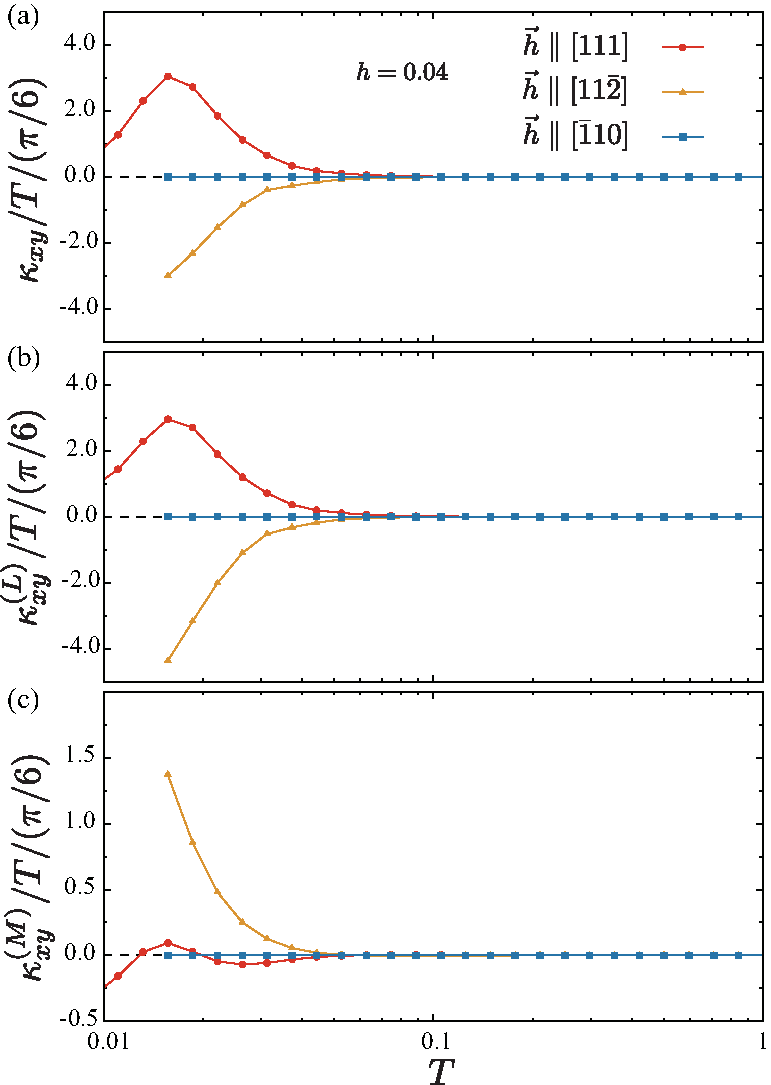
\includegraphics[width=0.9\linewidth]{Figs/plot_k_all_h0.04_ab.pdf}
  \end{center}
  \caption{(top) Temperature dependence of $\kappa_{xy}/T$ of the ferromagnetic Kitaev model under magnetic fields parallel to $[111]$, $[11\bar{2}]$, and $[\bar{1}10]$ with $|h|=0.04$. The horizontal dashed line indicates $\kappa_{xy}/T = 0$. The middle and the bottom figures are contributions from the three-body ($L$) and and the two-body ($M$) terms, respectively.}
  \label{fig:k_all_h0.04_ab}
\end{figure}

\begin{figure}
  \begin{center}
    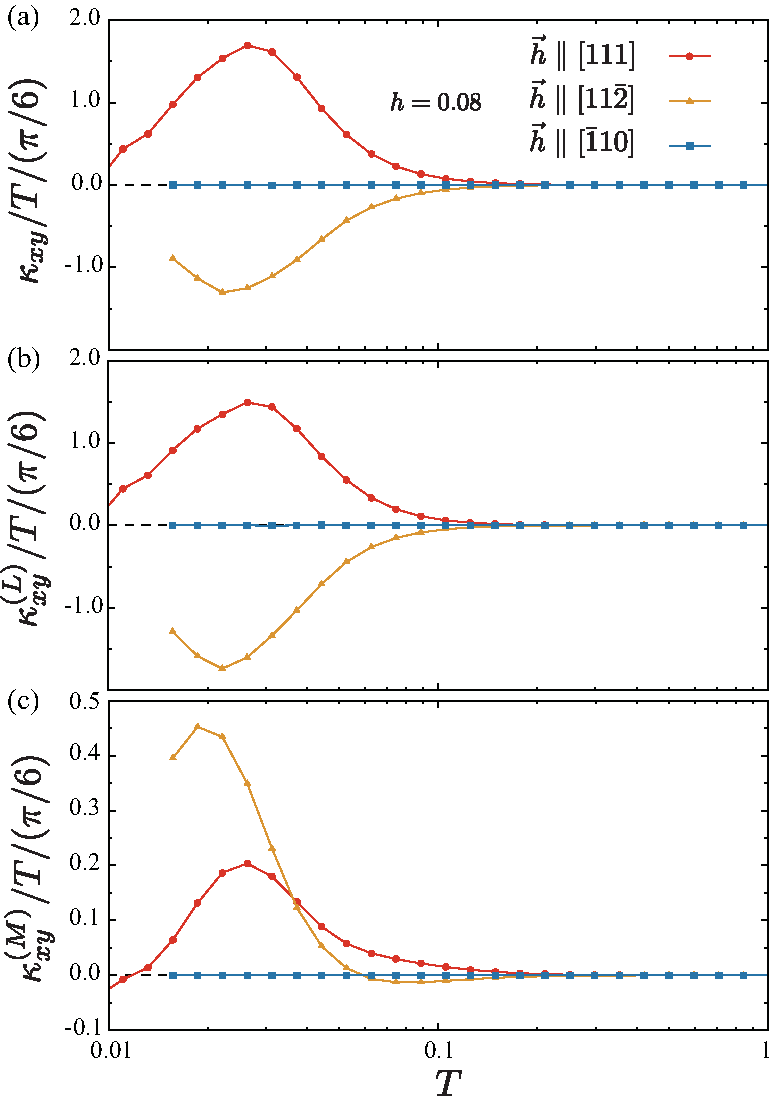
\includegraphics[width=0.9\linewidth]{Figs/plot_k_all_h0.08_ab.pdf}
  \end{center}
  \caption{(top) Temperature dependence of $\kappa_{xy}/T$ of the ferromagnetic Kitaev model under magnetic fields parallel to $[111]$, $[11\bar{2}]$, and $[\bar{1}10]$ with $|h|=0.08$. The horizontal dashed line indicates $\kappa_{xy}/T = 0$. The middle and the bottom figures are contributions from the three-body ($L$) and and the two-body ($M$) terms, respectively.}
  \label{fig:k_all_h0.08_ab}
\end{figure}
  \subsection{Effect of non-Kitaev interactions}
   As we discussed above, the thermal Hall conductivity of the pure Kitaev model shows a peak at a finite temperature, and its value largely overshoots the half-quantized value. Here, we investigate effect of the symmetry off-diagonal interactions, $\Gamma$ and $\Gamma'$ terms, to the thermal Hall transport.

   \subsubsection{Symmetric off-diagonal interaction $\Gamma$} 
   Firstly, we investigate the effect of $\Gamma$ interaction to $\kappa_{xy}/T$ under a magnetic field parallel to the $[111]$ direction. Again we consider two representative magnetic fields, $h=0.04$ and $h=0.08$.

In Figs.~\ref{fig:CMF_h0.04_G} and \ref{fig:CMF_h0.08_G}, we show temperature dependencies of the specific heat, the magnetization, and the flux for $\Gamma = 0, \pm 0.01, \pm 0.02$. Although $\Gamma$s are relatively small, we see significant change in the low-temperature peaks in the specific heat. For negative $\Gamma$, the peak moves to higher a temperature, and its height is enhanced. Similarly, the magnetization increases as for negative $\Gamma$. In the case of positive $\Gamma$, we observe the opposite effects, so that, the low-temperature peak of the specific heat moves lower temperature with decreasing its height, and magnetizations decreases. Both of negative and positive $\Gamma$s almost do not affect the high-temperature peak of the specific heat. We can also see sign dependent changes in the flux, although it is not so significant in the case of $h=0.04$ with positive $\Gamma$. 


\begin{figure}
  \begin{center}
    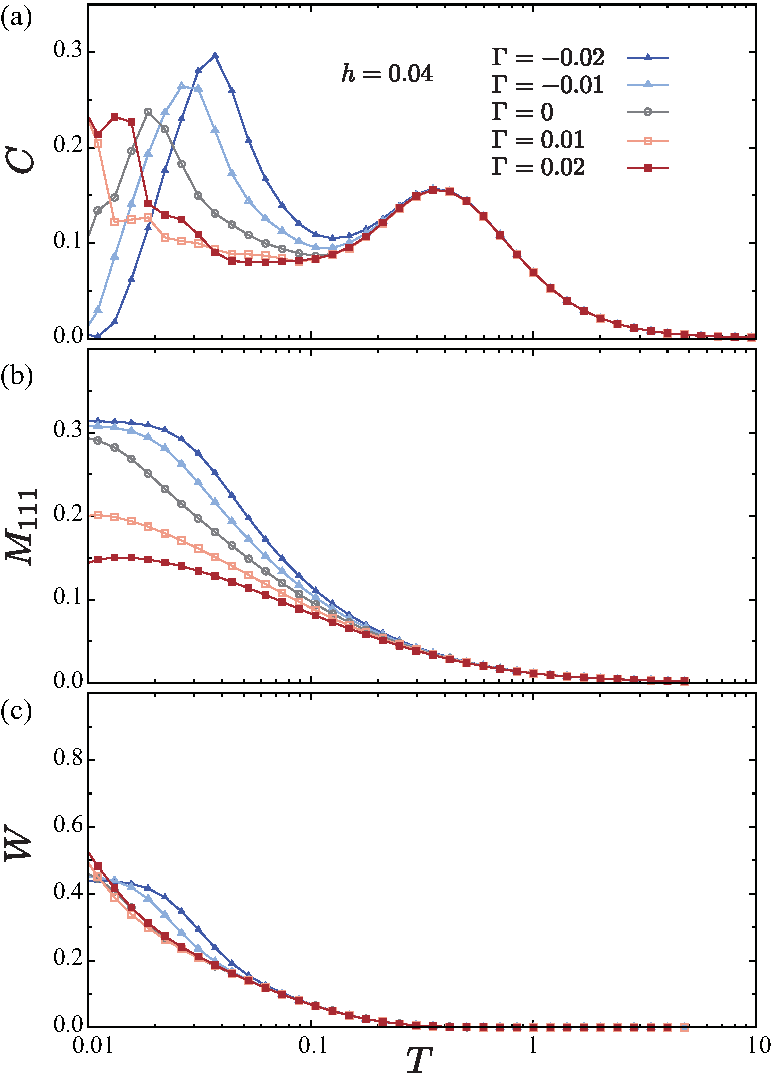
\includegraphics[width=0.9\linewidth]{Figs/plot_CMF_h0.04_G.pdf}
  \end{center}
  \caption{Temperature dependence of (a) the specific heat (b) the magnetic moment, and (c) the flux of the ferromagnetic Kitaev model with a weak $\Gamma$ under a magnetic field parallel to $[111]$ direction. The amplitude of the magnetic field is $|h|=0.04$.}
  \label{fig:CMF_h0.04_G}
\end{figure}
\begin{figure}
  \begin{center}
    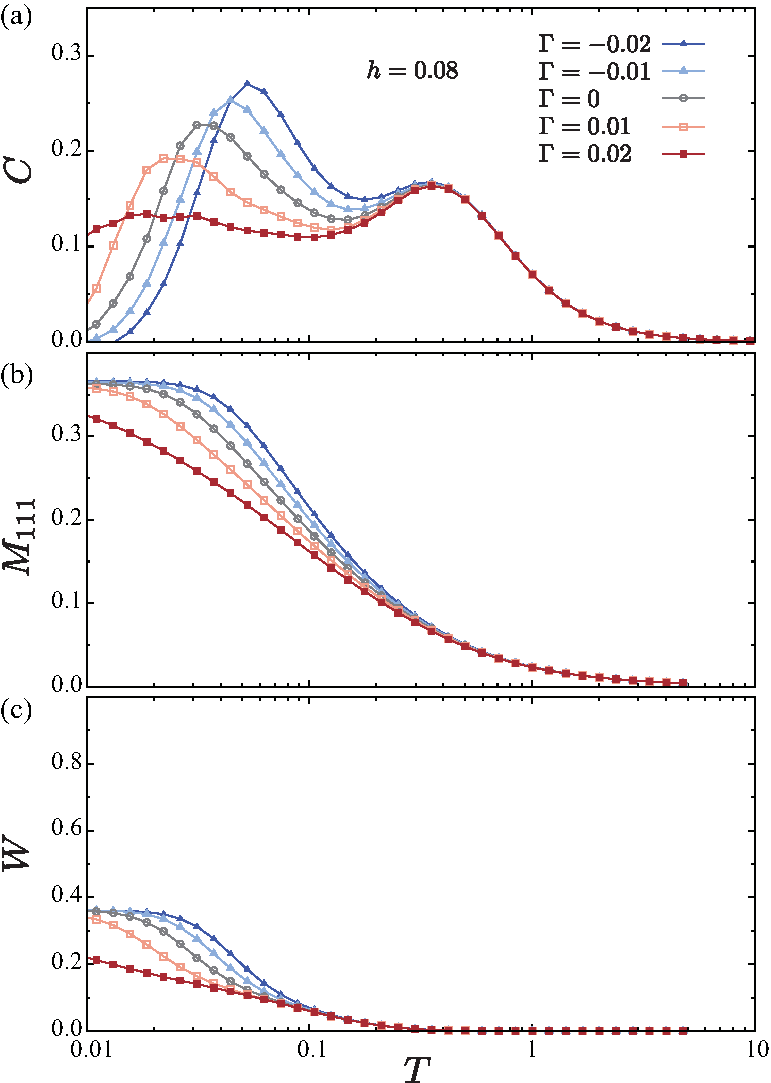
\includegraphics[width=0.9\linewidth]{Figs/plot_CMF_h0.08_G.pdf}
  \end{center}
  \caption{Temperature dependence of (a) the specific heat (b) the magnetic moment, and (c) the flux of the ferromagnetic Kitaev model with a weak $\Gamma$ under a magnetic field parallel to $[111]$ direction. The amplitude of the magnetic field is $|h|=0.08$.}
  \label{fig:CMF_h0.08_G}
\end{figure}

When we see $\kappa_{xy}/T$ shown in Figs.~\ref{fig:k_all_h0.04_G} and \ref{fig:k_all_h0.08_G}, we realize that the $\Gamma$ interaction can changes the thermal Hall transport significantly. Negative $\Gamma$ suppresses $\kappa_{xy}/T$ both for $h = 0.04$ and $h=0.08$. In the case of positive $\Gamma$, we see different behaviors between $h = 0.04$ and $h=0.08$. For $h=0.04$, positive $\Gamma$ suppresses $\kappa_{xy}/T$, and it becomes even negative for $\Gamma = 0.02$. In contrast to $h=0.04$, we see that positive $\Gamma$ enhances $\kappa_{xy}/T$. Such huge changes of $\kappa_{xy}/T$ by small $\Gamma$ seem to be different from the result of perturbation theory; it shows the contributions from $\Gamma$ appears as the third order\cite{YamadaF2021}. 

This magnetic field dependent behavior might be related to the relatively large $\kappa_{xy}^{(M)}/T$ for positive $\Gamma$. For $\Gamma \le 0$, the contributions from three-body correlation, $\kappa_{xy}^{L}$ dominate the total $\kappa_{xy}/T$. However, for $\Gamma = 0.01$ and $0.02$, the amplitudes of $\kappa_{xy}^{(M)}/T$ become larger, in particular for $\Gamma = 0.02$. This enhancement of the contribution from the two-body correlation might be related to nematic phases at the zero temperature observed in the infinite tensor network calculation \cite{LeeKCOYKK2020}.

\begin{figure}
  \begin{center}
    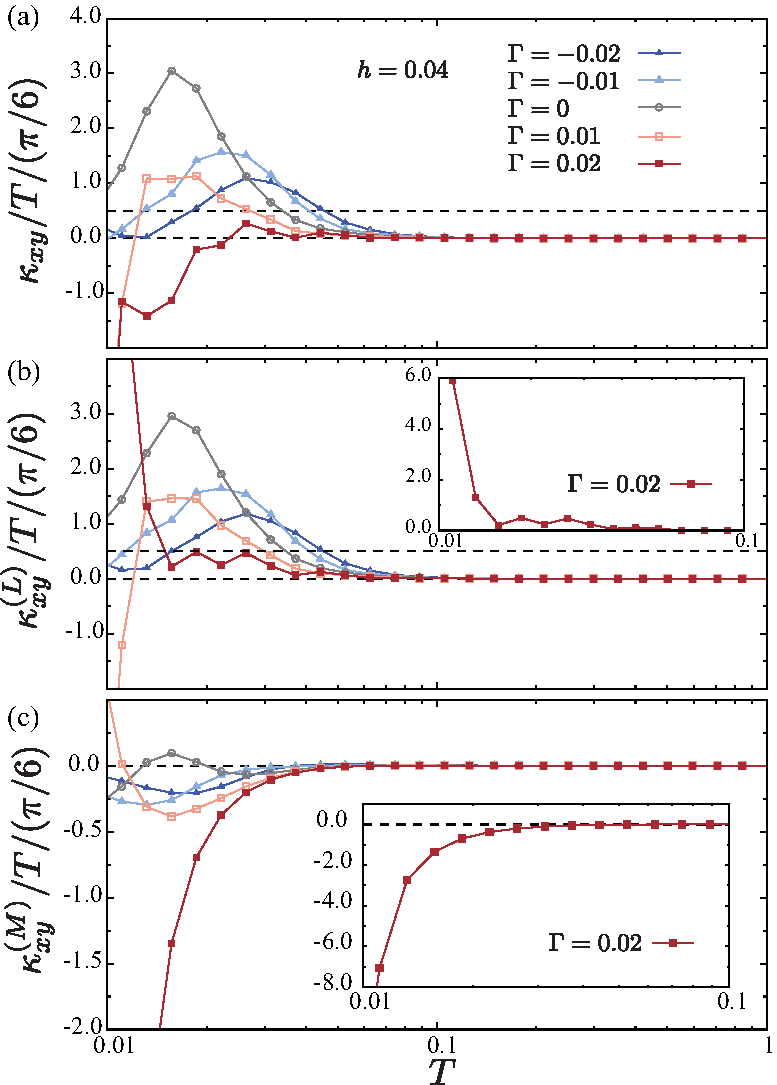
\includegraphics[width=0.9\linewidth]{Figs/plot_k_all_h0.04_G.pdf}
  \end{center}
  \caption{(a) Temperature dependence of $\kappa_{xy}/T$ of the ferromagnetic Kitaev model with as weak $\Gamma$ interaction under a magnetic field parallel to $[111]$. The amplitude of the magnetic field is set to $|h|=0.04$. Two horizontal dashed lines indicate $\kappa_{xy}/T = 0$ and the half-quantized value. (b, c) Contributions from the three-body ($L$) and and the two-body ($M$) terms, respectively.The insets show magnified views for $\Gamma = 0.02$.}
  \label{fig:k_all_h0.04_G}
\end{figure}
\begin{figure}
  \begin{center}
    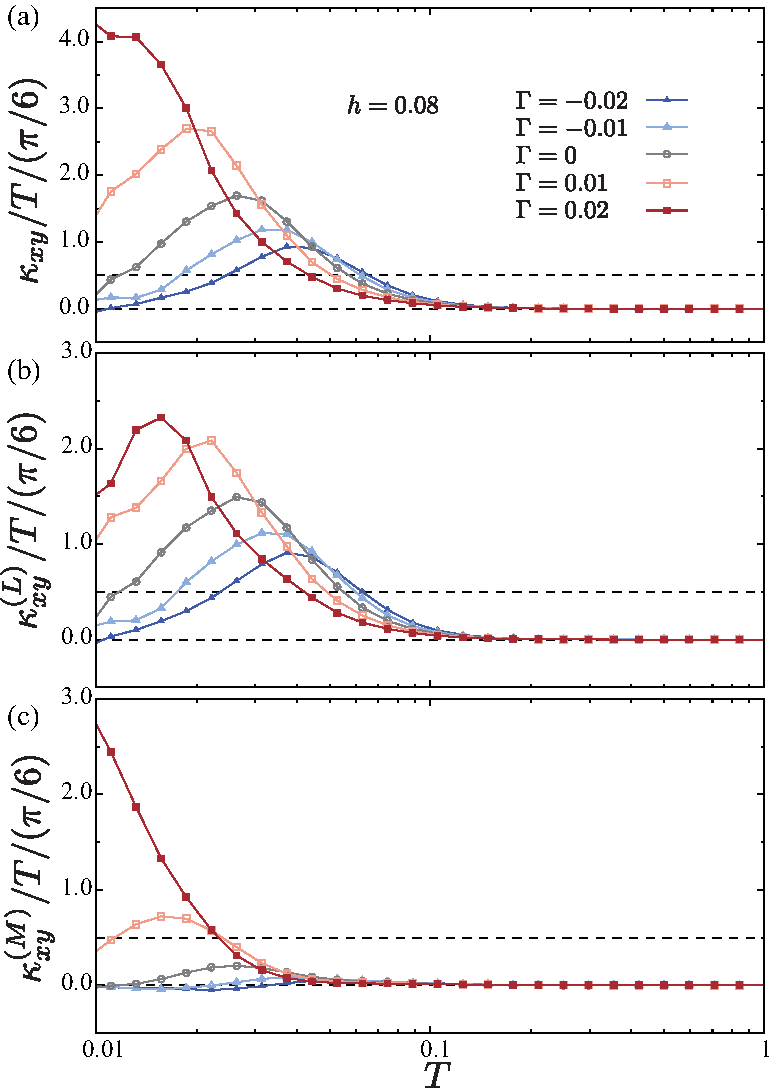
\includegraphics[width=0.9\linewidth]{Figs/plot_k_all_h0.08_G.pdf}
  \end{center}
  \caption{(a) Temperature dependence of $\kappa_{xy}/T$ of the ferromagnetic Kitaev model with as weak $\Gamma$ interaction under a magnetic field parallel to $[111]$. The amplitude of the magnetic field is set to $|h|=0.08$. Two horizontal dashed lines indicate $\kappa_{xy}/T = 0$ and the half-quantized value. (b, c) Contributions from the three-body ($L$) and and the two-body ($M$) terms, respectively.}
  \label{fig:k_all_h0.08_G}
\end{figure}
   
   

   \subsubsection{Symmetric off-diagonal interaction $\Gamma'$}
   Next, we consider the effect of $\Gamma'$ interaction to $\kappa_{xy}/T$ using two representative magnetic fields, $h=0.04$ and $h=0.08$. 
   
   In Figs.~\ref{fig:CMF_h0.04_Gp} and \ref{fig:CMF_h0.08_Gp}, we show several physical quantities for $\Gamma' = 0, \pm 0.01$, and $\pm 0.02$. We set, here, $\Gamma = 0$ to examine the pure effects of $\Gamma'$ term. Compared with $\Gamma$ terms, the specific-heat heights are almost unchnaged by $\Gamma'$, while low-temperatures peaks slightly move to higher or lower temperatures for negative and positive $\Gamma'$, respectively. Similar to the case of $\Gamma$ term, we see systematic change of the magnetization, although the observed changes are smaller than those in the case of $\Gamma$ (Fig.~\ref{fig:CMF_h0.04_ab} and \ref{fig:CMF_h0.04_ab}). Different from the $\Gamma$ term, the flux is almost unchanged by $\Gamma'$. 
\begin{figure}
  \begin{center}
    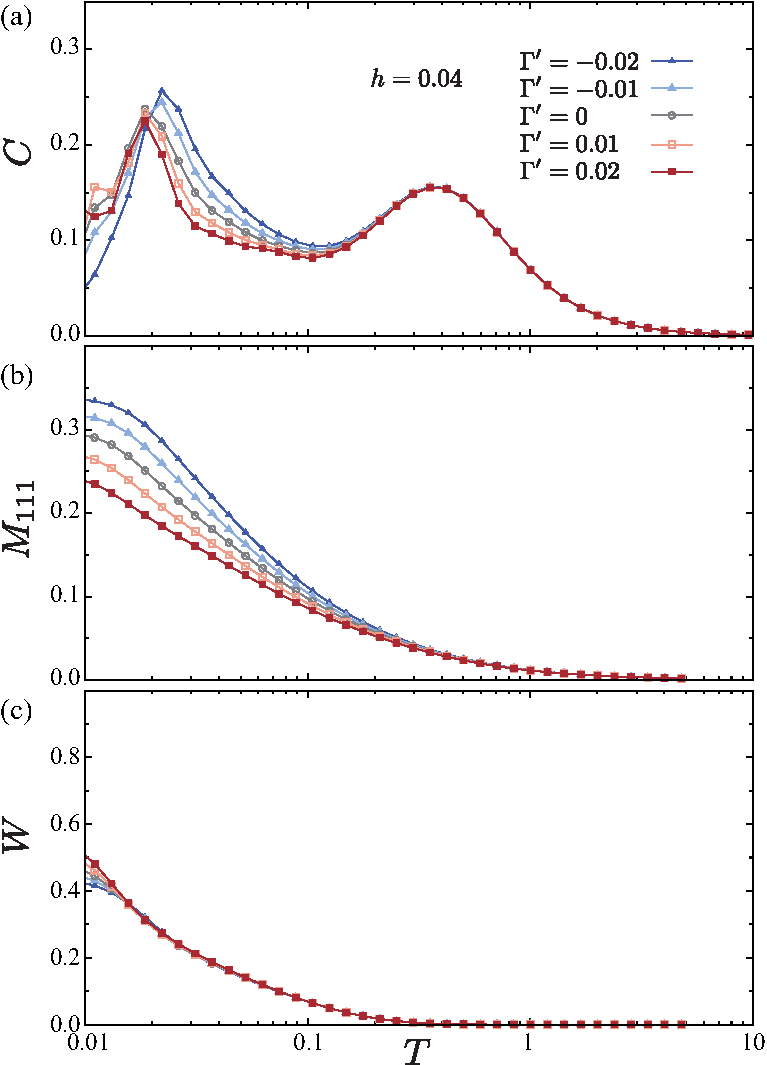
\includegraphics[width=0.9\linewidth]{Figs/plot_CMF_h0.04_Gp.pdf}
  \end{center}
  \caption{Temperature dependence of (a) the specific heat (b) the magnetic moment, and (c) the flux of the ferromagnetic Kitaev model with a weak $\Gamma'$ under a magnetic field parallel to $[111]$ direction. The amplitude of the magnetic field is $|h|=0.04$.}
  \label{fig:CMF_h0.04_Gp}
\end{figure}
\begin{figure}
  \begin{center}
    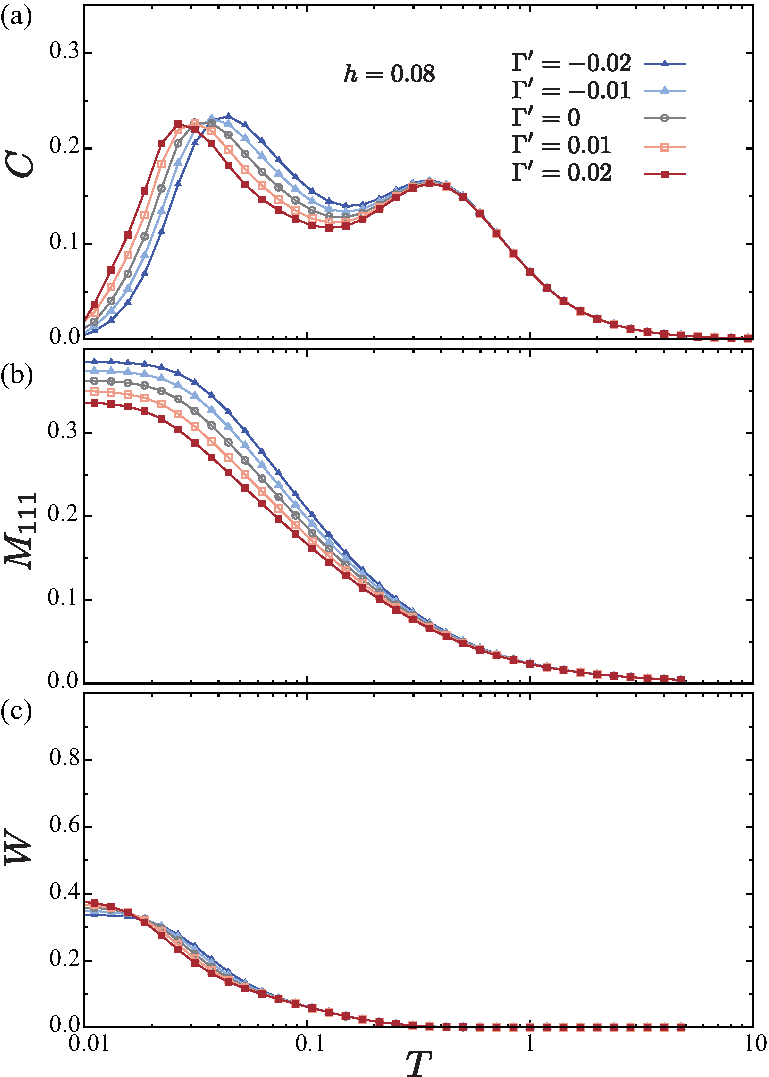
\includegraphics[width=0.9\linewidth]{Figs/plot_CMF_h0.08_Gp.pdf}
  \end{center}
  \caption{Temperature dependence of (a) the specific heat (b) the magnetic moment, and (c) the flux of the ferromagnetic Kitaev model with a weak $\Gamma'$ under a magnetic field parallel to $[111]$ direction. The amplitude of the magnetic field is $|h|=0.08$.}
  \label{fig:CMF_h0.08_Gp}
\end{figure}

 Figs.~\ref{fig:k_all_h0.04_Gp} and \ref{fig:k_all_h0.08_Gp} show temperature dependence of $\kappa_{xy}/T$ with the same $\Gamma'$s. Although the effects to the usual physical quantities are small as we saw above, $\Gamma'$ largely changes $\kappa_{xy}/T$; when we decrease $\Gamma'$, the peak of $\kappa_{xy}/T$ moves to higher temperature with increasing its height, while the peak moves to lower temperature with decreasing its height for positive \red{$\Gamma'$}. Such sign-dependent changes of $\kappa_{xy}$ somewhat consistent with the perturbation theory \cite{TakikawaF2020}. Note that correspondence between the peak temperature and the height is different from that for the $\Gamma$ (See Figs.~\ref{fig:k_all_h0.04_G}(a) and \ref{fig:k_all_h0.08_G}(a)). In the case of negative $\Gamma$ we observed that the peak moves higher temperature \textit{with decreasing its height}. Such qualitative difference might be useful to compare the present model calculation to experimental observations. 

Another important feature is negative $\kappa_{xy}/T$ observed at $\Gamma' = 0.02$ with $h = 0.04$. Although it is relatively small, we observe negative values both in $\kappa_{xy}^{(L)}/T$ and $\kappa_{xy}^{(M)}/T$. \textcolor{red}{In addition, we will see similar negative $\kappa_{xy}/T$ in the classical model (Need to check the classical counter part)}\blue{$\to$ Classicalの場合は、$\Gamma'$の方でのみ負になっています。古典系の部分では、$\Gamma'$導入の場合より$\Gamma$の方が量子性が効いていているのでは?という感じで書いていますが、ご検討お願いします}. Thus, we conclude that positive $\Gamma'$ can change the sign of $\kappa_{xy}/T$. 
\begin{figure}
  \begin{center}
    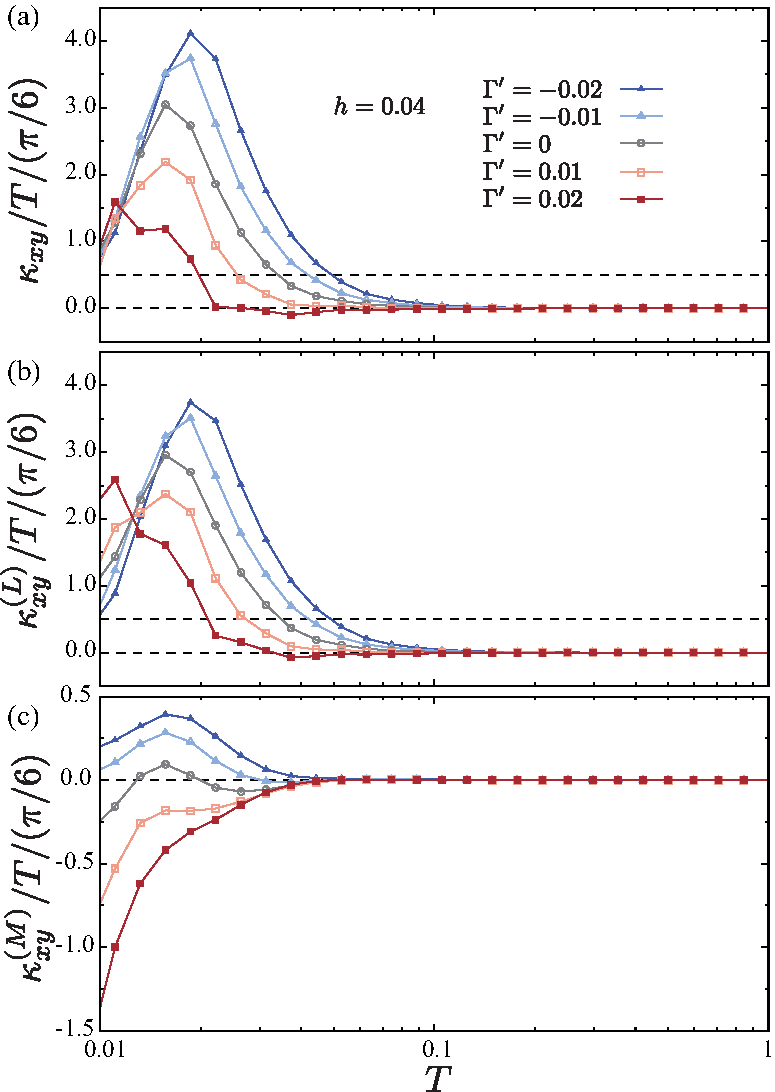
\includegraphics[width=0.9\linewidth]{Figs/plot_k_all_h0.04_Gp.pdf}
  \end{center}
  \caption{(a) Temperature dependence of $\kappa_{xy}/T$ of the ferromagnetic Kitaev model with as weak $\Gamma'$ interaction under a magnetic field parallel to $[111]$. The amplitude of the magnetic field is set to $|h|=0.04$. Two horizontal dashed lines indicate $\kappa_{xy}/T = 0$ and the half-quantized value. (b, c) Contributions from the three-body ($L$) and and the two-body ($M$) terms, respectively.}
  \label{fig:k_all_h0.04_Gp}
\end{figure}
\begin{figure}
  \begin{center}
    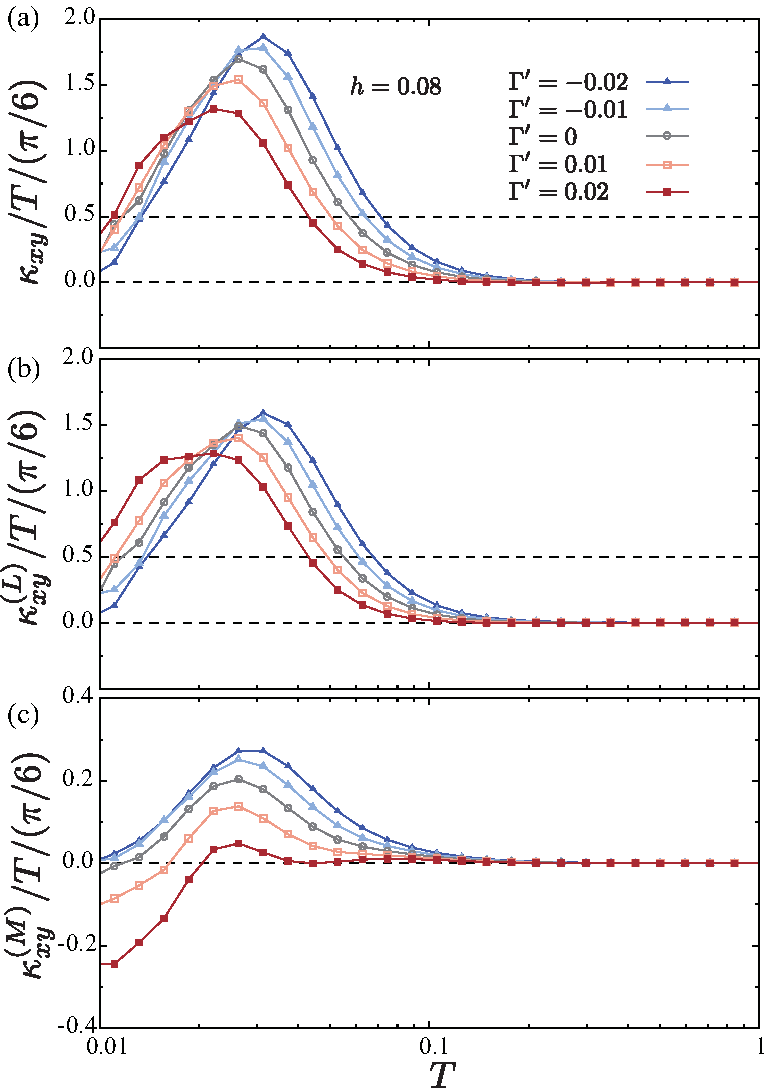
\includegraphics[width=0.9\linewidth]{Figs/plot_k_all_h0.08_Gp.pdf}
  \end{center}
  \caption{(a) Temperature dependence of $\kappa_{xy}/T$ of the ferromagnetic Kitaev model with as weak $\Gamma'$ interaction under a magnetic field parallel to $[111]$. The amplitude of the magnetic field is set to $|h|=0.08$. Two horizontal dashed lines indicate $\kappa_{xy}/T = 0$ and the half-quantized value. (b, c) Contributions from the three-body ($L$) and and the two-body ($M$) terms, respectively.}
  \label{fig:k_all_h0.08_Gp}
\end{figure}
 \subsection{Classical limit}

\begin{figure}[tbh] 
\begin{center} 
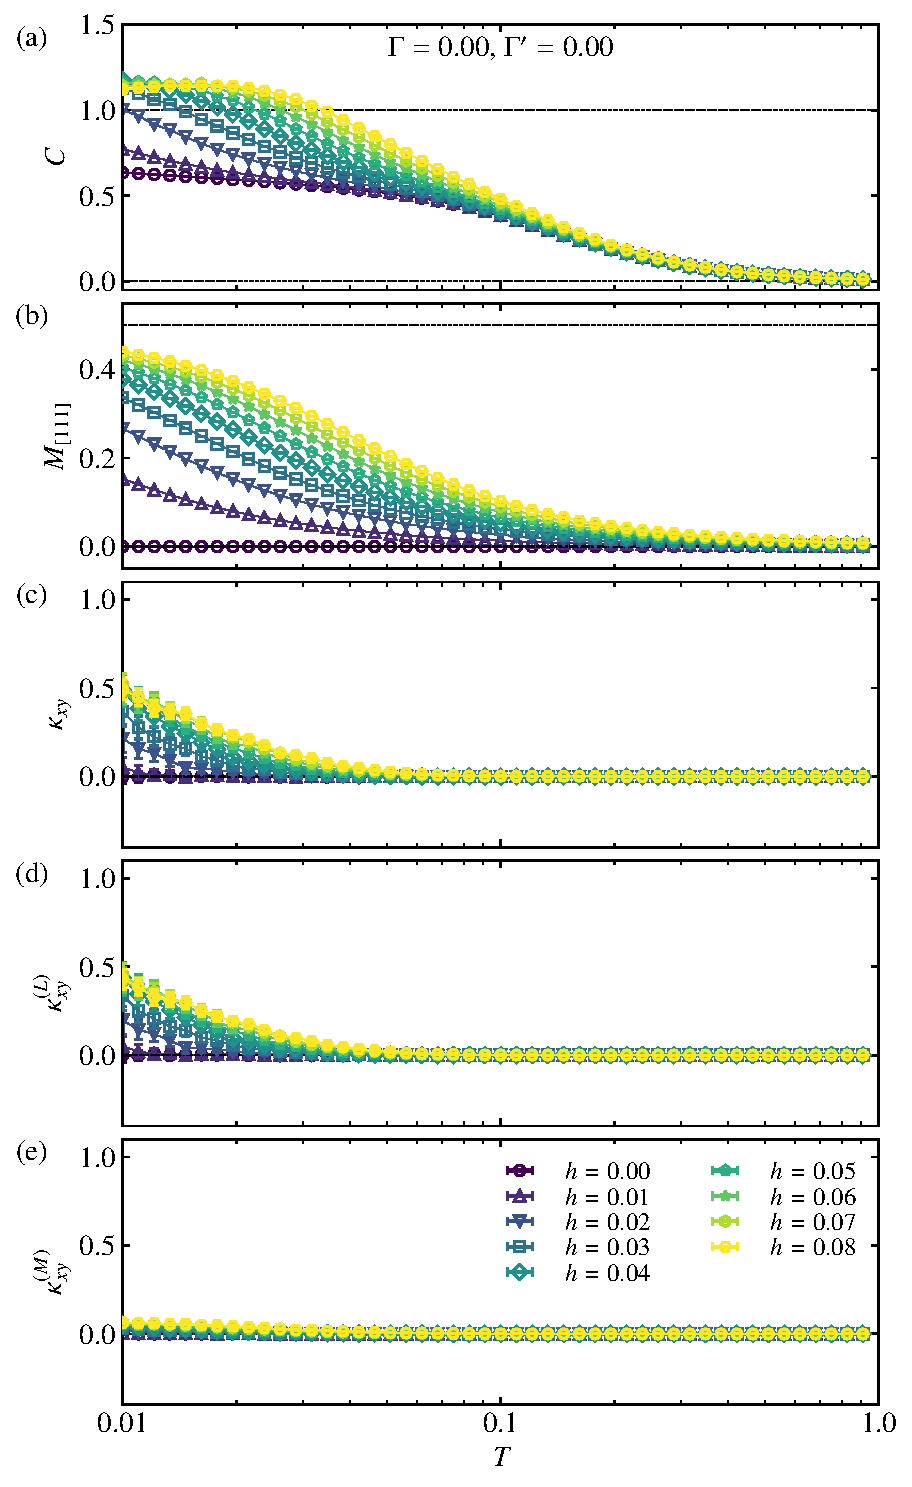
\includegraphics[width=0.9\linewidth]{Figs/fig_K-1.0_G0.00_Gp0.00_c.pdf}
\vspace{-0.5cm} 
\caption{Temperature dependence of (a) the specific heat, (b) the total magnetization, and
(c) the thermal Hall conductivity $\kappa_{xy}$ for several magnetic fields along the $[111]$ direction in the classical Kitaev model.
(d),(e) Temperature dependence of the two components, $(L)$ and $(M)$, of the thermal Hall conductivity.}
\label{fig_classical_hdep}
\end{center}
\end{figure}

In this section, we show the results obtained by applying the classical approximation for \blue{Eq.~\eqref{eq:model-Hamiltonian}} to compare those for the quantum spin model shown above.
First, we focus on the pure Kitaev model with $\Gamma=\Gamma'=0$.
Figure~\ref{fig_classical_hdep}(a) shows the temperature dependence of the specific heat of the classical Kitaev model at several magnetic fields along the $[111]$ direction.
In the absence of the magnetic field, the previous studies clarified that the specific heat monotonically increases with decreasing temperature and approaches $3/4$ in the zero temperature limit\blue{~\cite{Sela2014,suzuki2018}}.
This value originates from the zero modes intrinsic to the pure Kitaev model without magnetic field, and the quartic order of the spin fluctuations contributes to the specific heat at $T\to 0$.
Once the magnetic field is introduced, it lifts the zero modes, and thereby, the zero-$T$ limit of the specific heat takes the conventional value, i.e., 1, owing to the presence of the two continuous variables $(\theta,\phi)$ at each site.
We find that it shows a peak at the temperature corresponding to the energy scale of $h$ in the presence of the magnetic field despite the monotonic change at $h=0$.
In this temperature scale, the magnetization develops, as shown in Fig.~\ref{fig_classical_hdep}(b).

Figure~\ref{fig_classical_hdep}(c) shows the thermal Hall conductivity as a function of temperature.
When the magnetic field is not applied, this is always zero.
By introducing the magnetic field, $\kappa_{xy}$ becomes nonzero and is positive, which is consistent with the results for the quantum system.
Moreover, the temperature scale for developing the thermal Hall conductivity is much smaller than that for the magnetization.
The distinctly different temperature scales appear to be similar to those in the quantum system [see Figs.~\ref{fig:CMF_pure} and \ref{fig:k_all_pure}] although the double-peak structure of the specific heat is not observed in the classical system.
In the classical result, $\kappa_{xy}$ shows a monotonic increase with decreasing temperature.
On the other hand, in the quantum system, $\kappa^{xy}/T$ takes a peak around the temperature at which the specific heat exhibits the low-$T$ peak, as shown in Fig.~\ref{fig:k_all_pure}.
The difference is considered to originate from an artifact in the classical system, where the macroscopic degeneracy is present in the low-energy region leading to the nonzero specific heat at zero temperature.
\blue{Thus, the quantization of $\kappa^{xy}/T$ does not occur in the classical system.}
Figures~\ref{fig_classical_hdep}(d) and \ref{fig_classical_hdep}(e) present the three-body and two-body contributions of the thermal current to the thermal Hall conductivity, respectively.
The two-body contributions $\kappa_{xy}^{(M)}$ is much smaller than the three-body one $\kappa_{xy}^{(L)}$, indicating that the thermal Hall effect is dominated by the three-body terms of the thermal current at the edges.
\blue{This result is consistent with the quantum system, but the classical approximation appears not to reproduce small negative values of $\kappa_{xy}^{(M)}$ in weak magnetic fields as shown in Fig.~\ref{fig:k_all_pure}(c).}


\begin{figure}[tbh] 
\begin{center} 
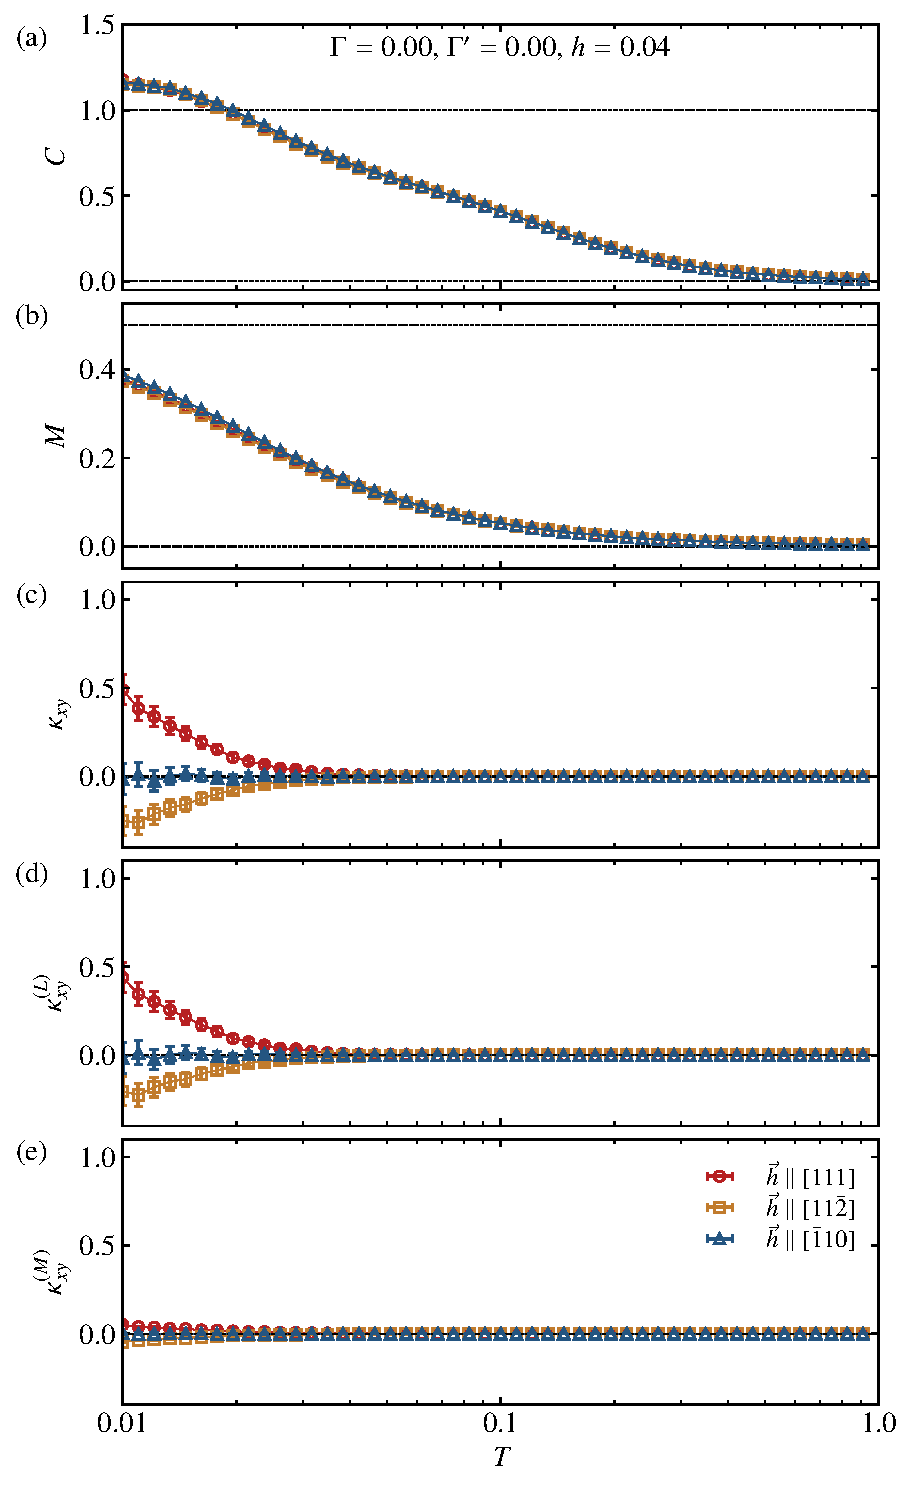
\includegraphics[width=0.9\linewidth]{Figs/fig_K-1.0_G0.00_Gp0.00_h0.04.pdf}
\vspace{-0.5cm} 
\caption{Temperature dependence of (a) the specific heat, (b) the total magnetization, and
(c) the thermal Hall conductivity $\kappa_{xy}$ in the classical Kitaev model under the magnetic field parallel to $[111]$, $[11\bar{2}]$, and $[\bar{1}10]$ with $h=0.04$.
(d),(e) Temperature dependence of the two components, $(L)$ and $(M)$, of the thermal Hall conductivity.}
\label{fig_classical_adep004}
\end{center}
\end{figure}
  

Next, we discuss the field-angle dependence in the pure Kitaev model.
We consider the three field directions $[11\bar{2}]$, $[\bar{1}10]$, and $[111]$, which are perpendicular to each other.
Figures~\ref{fig_classical_adep004}(a) and \ref{fig_classical_adep004}(b) show the temperature dependence of the specific heat and magnetization along the corresponding field direction.
These indicate that the field direction hardly changes the specific heat and magnetization, which is also observed in the quantum system \red{(See Figs.~\ref{fig:CMF_h0.04_ab} and \ref{fig:CMF_h0.04_ab})}. \blue{[図がないので大久保さんの方で確認お願いします]}\red{(実は、appendixに置いてありました。最終的にどうするかわからないですが、とりあえずその図を参照。)}.
On the other hand, the thermal Hall conductivity strongly depends on the direction of the applied magnetic field.
As shown in Figure~\ref{fig_classical_adep004}(c), $\kappa_{xy}$ is negative and decreases with deceasing temperature for $\vec{h}\parallel [11\bar{2}]$ in contrast to the case with $\vec{h}\parallel [111]$.
Moreover, the absolute value for the former is smaller than that for the latter.
While these characteristics are consistent with that in the quantum system, the peak structure in Fig.~\ref{fig:k_all_h0.04_ab}(a) is not seen in the classical case.
Furthermore, a large enhancement of $\kappa_{xy}^{(M)}$ at low temperatures for $\vec{h}\parallel [11\bar{2}]$ presented in Fig.~\ref{fig:k_all_h0.04_ab}(c) is not reproduced in the classical system as shown in Fig.~\ref{fig_classical_adep004}(e) despite the similarity for the temperature of $\kappa_{xy}^{(L)}$ in the quantum and classical systems [Figs.~\ref{fig:k_all_h0.04_ab}(b) and \ref{fig_classical_adep004}(d)].
This result suggests that the three-body term can be understood in the classical picture, but quantum fluctuations beyond the classical approach substantially contributes to the two-body term.
% \red{[2体項はtime-reversal evenで、磁場によって古典的に誘発されたものではないから??]}
% \red{[以下は、量子系のところに入れた方が良いかも]}
We also find that the thermal Hall conductivity is zero in the magnetic field applied along the $[\bar{1}10]$ direction\blue{, which results in the symmetry of the Hamiltonian, as discussed before.}
% This is understood from the fact that the Hamiltonian is invariant under the following two operations simultaneously:
% The $C_2$ rotation along the $[\bar{1}10]$ axis in the spin space transferring $(S^x,S^y,S^z)$ to $(-S^y,-S^x,-S^z)$ and the rotation of the honeycomb plane along the $z$~bond in the real space, which exchanges the $x$ and $y$~bonds.
% However, the rotation of the honeycomb plane inverts the component along the zigzag edge of the position vector $\bm{r}$, and thereby, the thermal current along the zigzag edge should be zero.
% Note that the above argument is applicable in the presence of the $\Gamma$ and $\Gamma'$ interactions.



% \begin{figure}[tbh] 
%   \begin{center} 
%   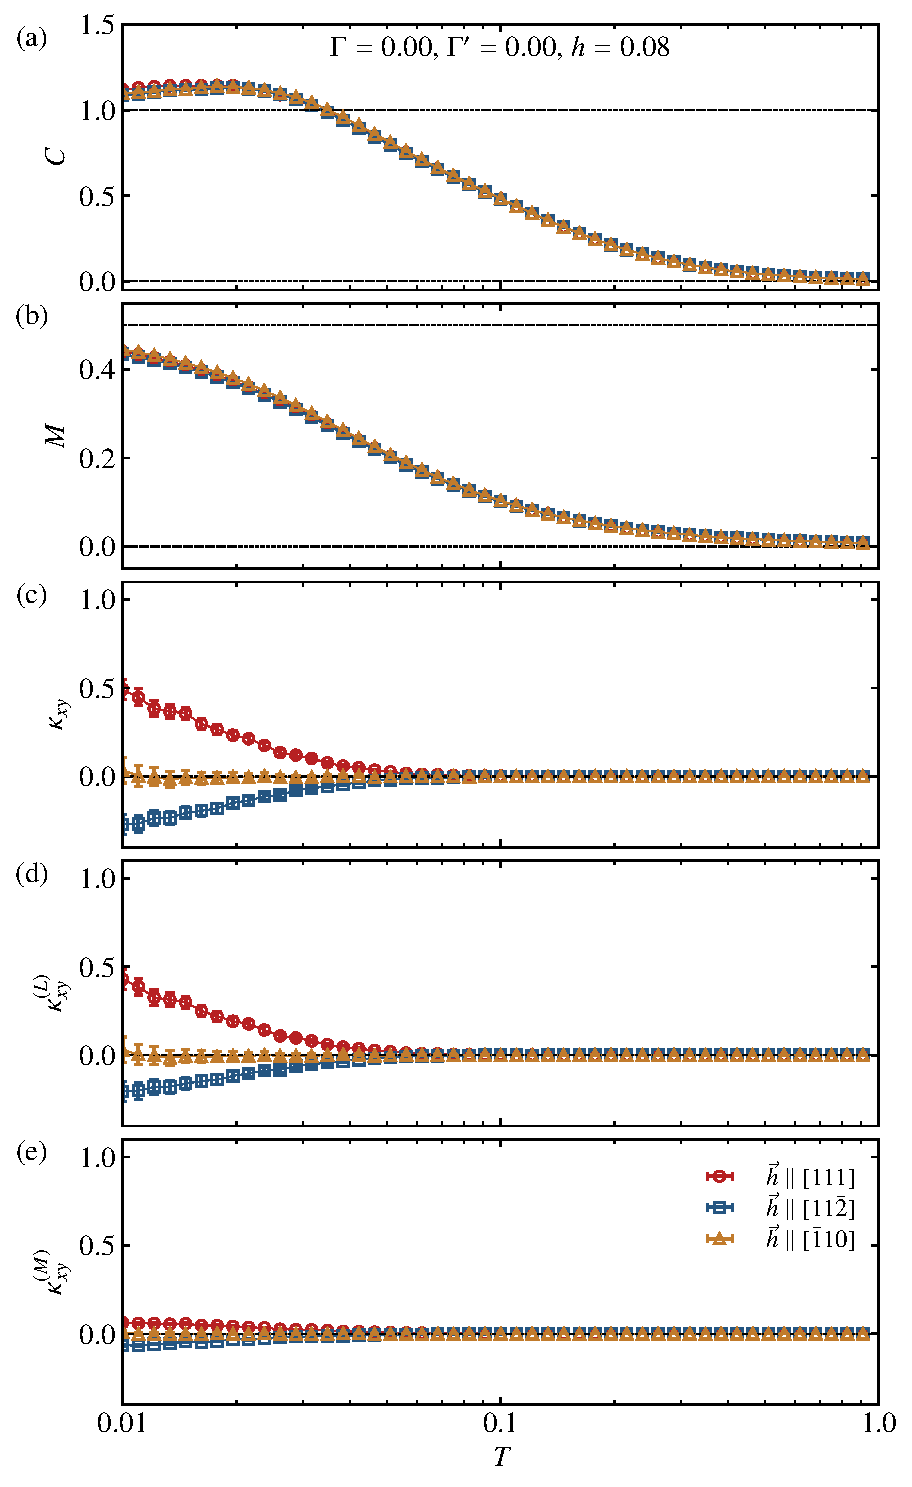
\includegraphics[width=0.9\linewidth]{fig_K-1.0_G0.00_Gp0.00_h0.08.pdf}
%   \vspace{-0.5cm} 
%   \caption{Temperature dependence of (a) the specific heat, (b) the total magnetization, and
%   (c) the thermal Hall conductivity $\kappa_{xy}$ in the classical Kitaev model under the magnetic field parallel to $[111]$, $[11\bar{2}]$, and $[\bar{1}10]$ with $h=0.08$.
%   (d),(e) Temperature dependence of the two components, $(L)$ and $(M)$, of the thermal Hall conductivity.}
%   \label{fig_classical_adep008}
%   \end{center}
%   \end{figure}




\begin{figure}[tbh] 
\begin{center} 
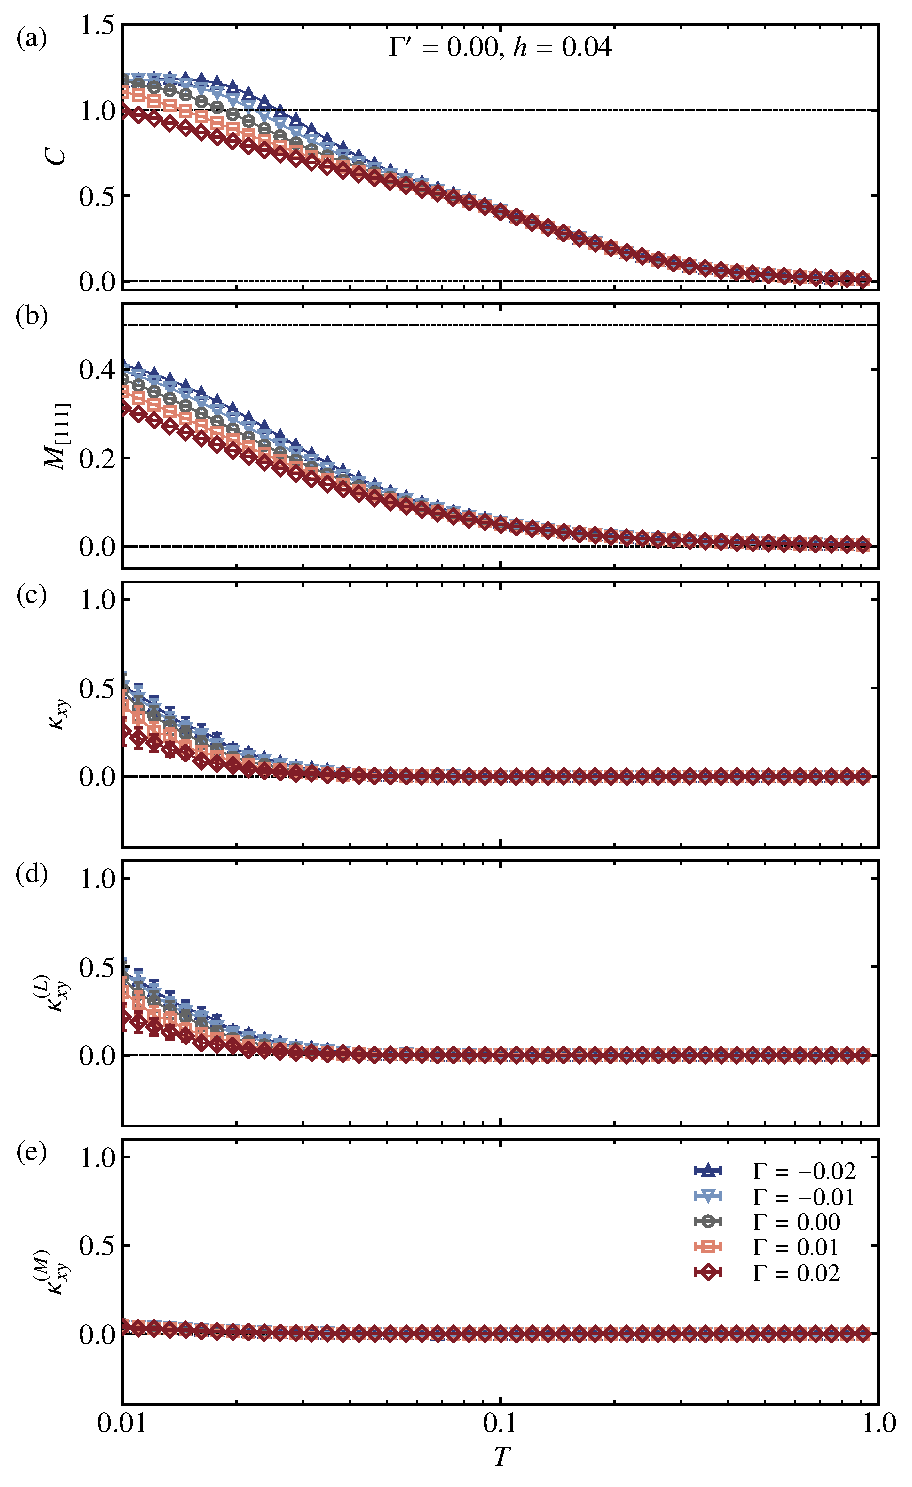
\includegraphics[width=0.9\linewidth]{Figs/fig_K-1.0_Gp0.00_h0.04.pdf}
\vspace{-0.5cm} 
\caption{Temperature dependence of (a) the specific heat, (b) the total magnetization, and
(c) the thermal Hall conductivity $\kappa_{xy}$ in the classical Kitaev-$\Gamma$ model under the magnetic field with $h=0.04$.
(d),(e) Temperature dependence of the two components, $(L)$ and $(M)$, of the thermal Hall conductivity.}
\label{fig_classical_gdep004}
\end{center}
\end{figure}


Here, we introduce the $\Gamma$ and $\Gamma'$ interactions in the Kitaev model.
First, we focus on the effect of the $\Gamma$ term.
Figure~\ref{fig_classical_gdep004} shows the temperature dependence of physical quantities at several values of $\Gamma$ with $\Gamma'=0$.
\blue{For the case of the negative $\Gamma$, the low-$T$ specific heat is enhanced with increasing the absolute value of $\Gamma$ as shown in Fig.~\ref{fig_classical_gdep004}(a).
On the other hand, the specific heat is suppressed by the introduction of the positive $\Gamma$.
These tendencies are consistent with the results in the quantum system while peak structure shown in Fig.~\ref{fig:CMF_h0.04_G}(a) is not reproduced in the classical simulations.
Figure~\ref{fig_classical_gdep004}(b) shows the temperature dependence of the magnetization at several $\Gamma$.
The magnetization increases with decreasing $\Gamma$, which is also observed in the quantum result shown in Fig.~\ref{fig:CMF_h0.04_G}(b).
}
% A peak in the specific heat is shifted to the high-temperature side with increasing the absolute value of $\Gamma$ for $\Gamma<0$.
% In the case of the positive $\Gamma$, the specific heat is suppressed by increasing $\Gamma$.
% The magnetization is suppressed for $\Gamma>0$ but is enhanced for $\Gamma<0$, as shown in Fig.~\ref{fig_classical_gdep004}(b).
% This tendency is observed also in $\kappa_{xy}$,
\blue{This $\Gamma$ dependence is also seen in $\kappa_{xy}$,}
which is dominated by the three-body contribution [Figs.~\ref{fig_classical_gdep004}(c)--\ref{fig_classical_gdep004}(e)].
% While the temperature dependence of the specific heat and magnetization is consistent with that in the quantum system [Figs.~\ref{fig:CMF_h0.04_G}(a) and \ref{fig:CMF_h0.04_G}(b)],
\blue{While a similar $\Gamma$ dependence is observed in the specific heat and magnetization for the quantum system [Figs.~\ref{fig:CMF_h0.04_G}(a) and \ref{fig:CMF_h0.04_G}(b)],}
 the low-temperature behavior of the thermal Hall conductivity is different from that in the quantum system shown in Fig.~\ref{fig:k_all_h0.04_G}.
The characteristic feature of the results for the quantum system is the substantial enhancement of $\kappa_{xy}^{(L)}$ and $\kappa_{xy}^{(M)}$, which are almost canceled out in the total thermal Hall conductivity $\kappa_{xy}$.
This is not reproduced in the classical system, suggesting that it is yielded by quantum fluctuations.
Nevertheless, in the intermediate temperature region around $T=0.05$ in Fig.~\ref{fig:k_all_h0.04_G}, the $\Gamma$ and temperature dependencies are similar to the low-temperature behavior in the classical system shown in Figs.~\ref{fig_classical_gdep004}(c)--\ref{fig_classical_gdep004}(e).
These results imply that the behavior in the temperature region of the quantum system is understood by the classical regime.


% \begin{figure}[tbh] 
% \begin{center} 
% 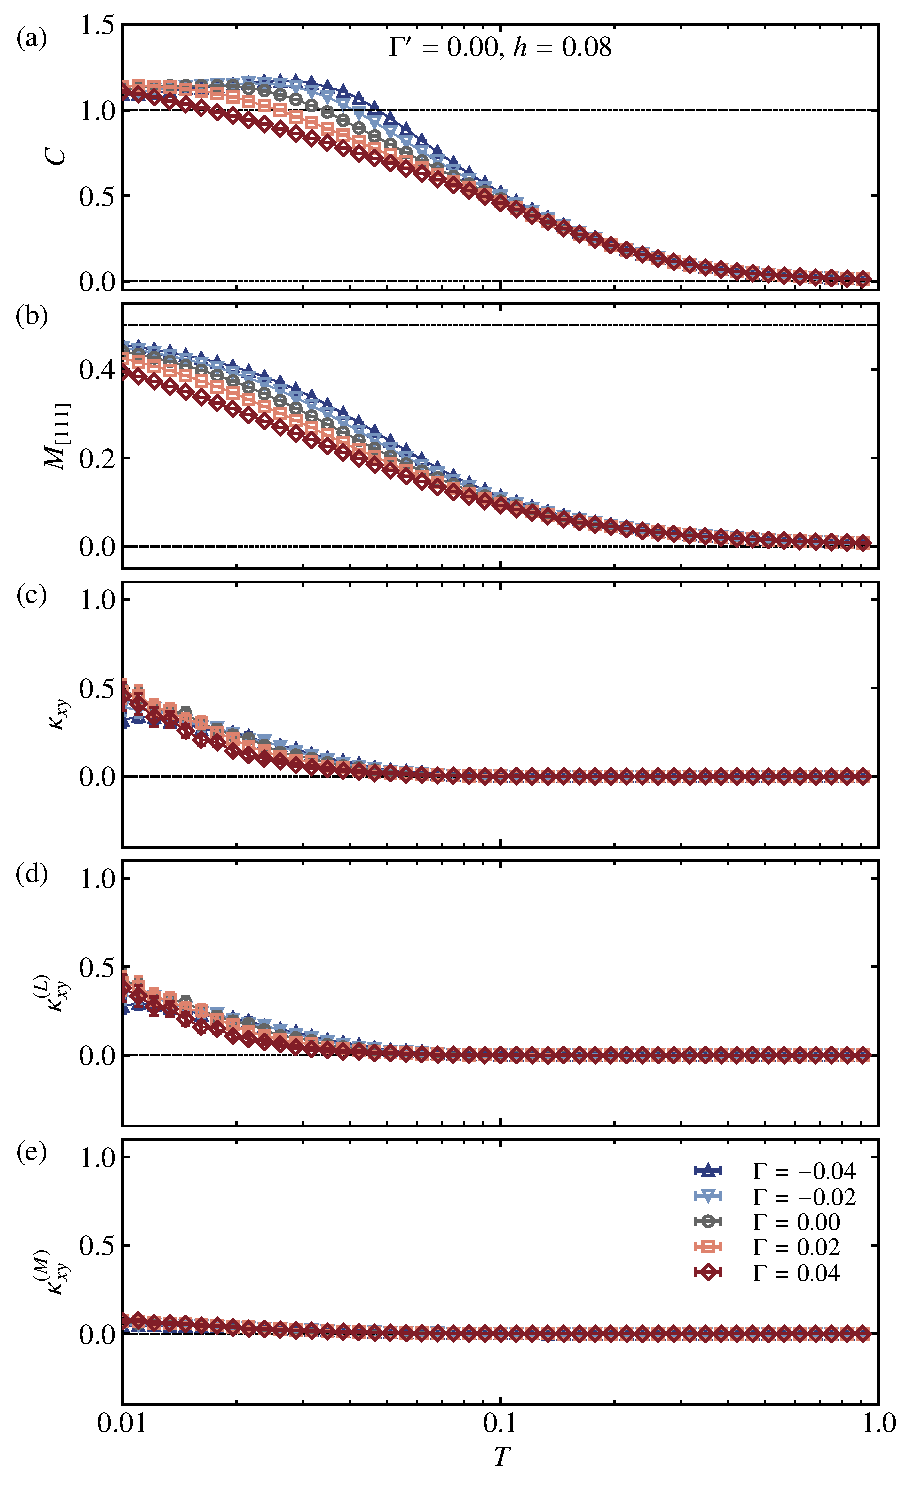
\includegraphics[width=0.9\linewidth]{fig_K-1.0_Gp0.00_h0.08.pdf}
% \vspace{-0.5cm} 
% \caption{Temperature dependence of (a) the specific heat, (b) the total magnetization, and
% (c) the thermal Hall conductivity $\kappa_{xy}$ in the classical Kitaev-$\Gamma$ model under the magnetic field with $h=0.08$.
% (d),(e) Temperature dependence of the two components, $(L)$ and $(M)$, of the thermal Hall conductivity.}
% \label{fig_classical_gdep008}
% \end{center}
% \end{figure}
  


\begin{figure}[tbh] 
\begin{center} 
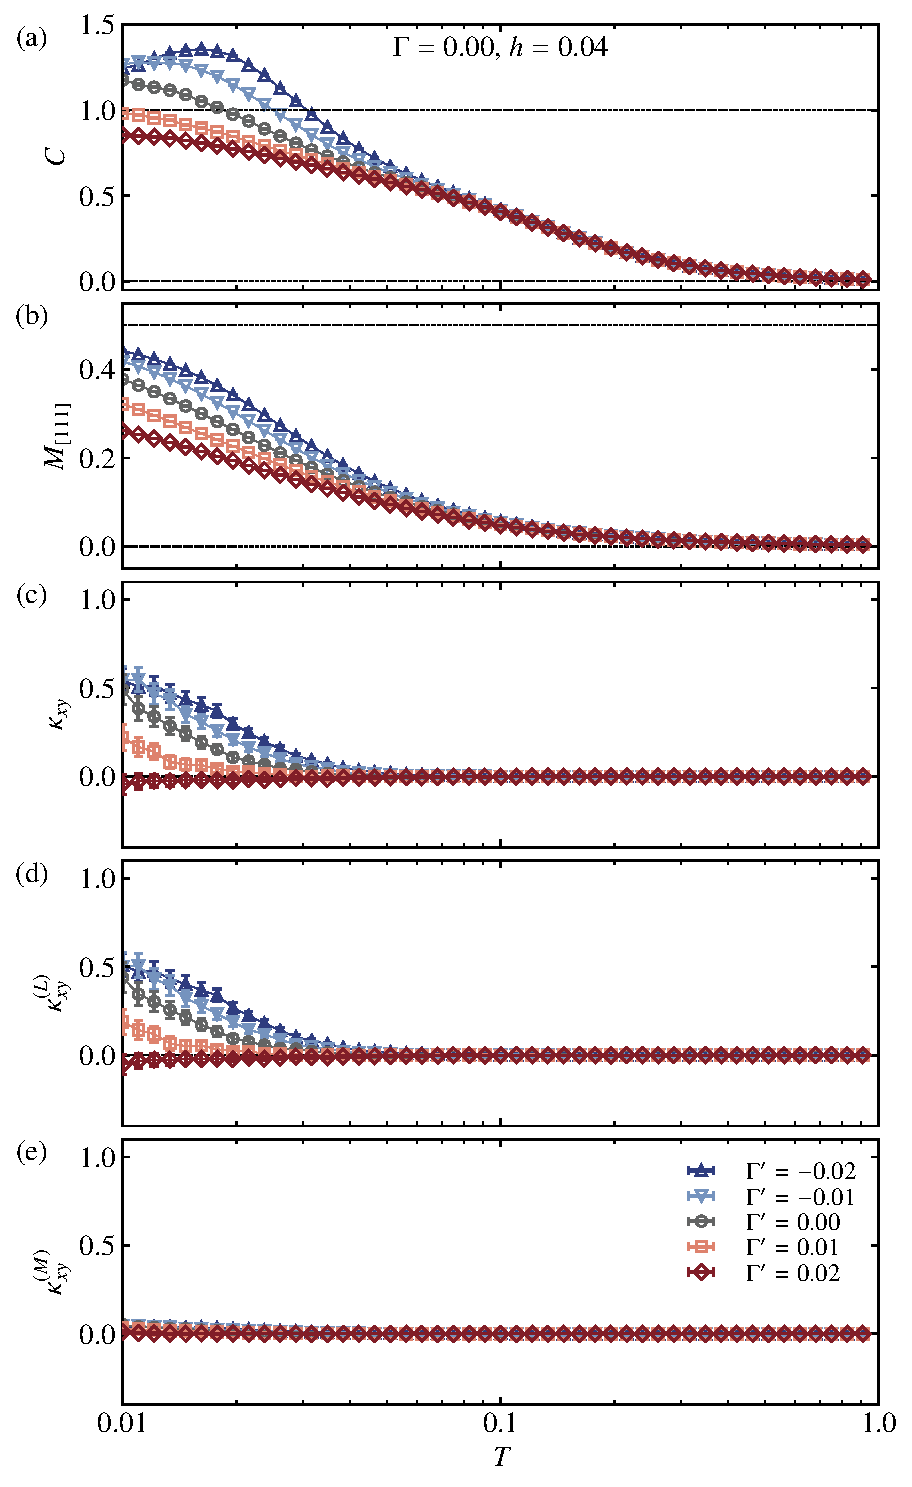
\includegraphics[width=0.9\linewidth]{Figs/fig_K-1.0_G0.00_h0.04.pdf}
\vspace{-0.5cm} 
\caption{Temperature dependence of (a) the specific heat, (b) the total magnetization, and
(c) the thermal Hall conductivity $\kappa_{xy}$ in the classical Kitaev-$\Gamma'$ model under the magnetic field with $h=0.04$.
(d),(e) Temperature dependence of the two components, $(L)$ and $(M)$, of the thermal Hall conductivity.}
\label{fig_classical_gpdep004}
\end{center}
\end{figure}

Finally, we examine the effect of the $\Gamma'$ interaction on the Kitaev system.
Figure~\ref{fig_classical_gpdep004} shows the temperature dependence of physical quantities for several values of $\Gamma'$ in the Kitaev-$\Gamma'$ model without the $\Gamma$ interaction.
The positive $\Gamma'$ suppresses the specific heat and magnetization while the negative $\Gamma'$ enhances them.
Moreover, we find a peak in the specific heat at $\Gamma'=-0.02$ in Fig.~\ref{fig_classical_gpdep004}, \blue{indicating} its shift to the high-temperature side with decreasing $\Gamma'$.
These tendencies are also seen in the quantum system, as shown in Figs.~\ref{fig:CMF_h0.04_Gp}(a) and \ref{fig:CMF_h0.04_Gp}(a).
\blue{Meanwhile, we also find inconsistent behavior in the difference from the effect on the $\Gamma$ interaction.
For the classical simulations, the specific heat and magnetization appear to be sensitive to $\Gamma'$ rather than $\Gamma$, which is opposite to results in the quantum system (Figs.~\ref{fig:k_all_h0.04_G} and \ref{fig:k_all_h0.04_Gp}).
This contrasting behavior suggests that the $\Gamma'$ interaction stabilizes spin states with weak quantum fluctuations, but the $\Gamma$ one enhances quantum effects.
Indeed, it has been pointed out that the $\Gamma$ interaction does not destroy a QSL state~\cite{Gohlke2018,catuneanu2018}, whereas the introduction of $\Gamma'$ shrinks the region of the QSL phase~\cite{gordon2019theory,Luo2022}.
}
For the thermal transport, we find that the positive $\Gamma'$ suppresses the thermal Hall conductivity, and it becomes negative at low temperatures in the classical system [Fig.~\ref{fig_classical_gpdep004}(c)].
The three-body part dominantly contributes to the thermal Hall conductivity, as shown in Figs.~\ref{fig_classical_gpdep004}(d) and \ref{fig_classical_gpdep004}(e).
Here, we compare the above results with those in the quantum system presented in Fig.~\ref{fig:k_all_h0.04_Gp}.
As discussed \blue{before,} %in the previous paragraph for the $\Gamma$ dependence,
results for the classical limit should be compared with those for the intermediate temperature range ($T\sim 0.05$) in the quantum system.
Although the thermal Hall conductivity in this system takes a positive value at the lowest temperature [Fig.~\ref{fig:k_all_h0.04_Gp}(a)], it appears to be negative in the intermediate temperature range.
Moreover, in this temperature range, $\kappa_{xy}^{(M)}$ is much smaller than $\kappa_{xy}^{(M)}$, as shown in Figs.~\ref{fig:k_all_h0.04_Gp}(b) and \ref{fig:k_all_h0.04_Gp}(c), which are consistent with the corresponding results for the classical system.


% \begin{figure}[tbh] 
% \begin{center} 
% 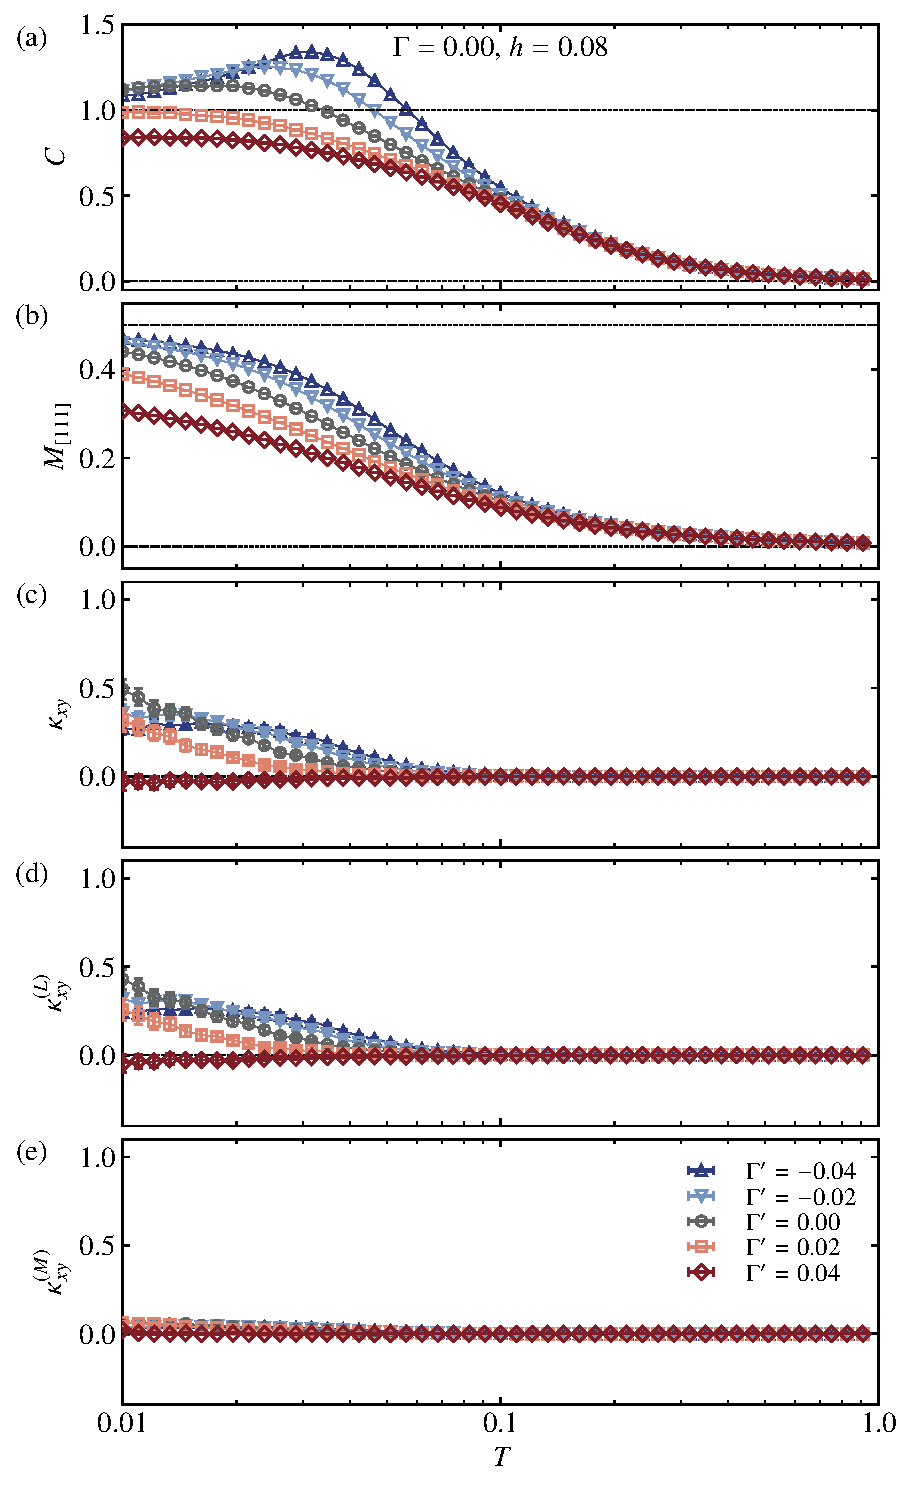
\includegraphics[width=0.9\linewidth]{fig_K-1.0_G0.00_h0.08.pdf}
% \vspace{-0.5cm} 
% \caption{Temperature dependence of (a) the specific heat, (b) the total magnetization, and
% (c) the thermal Hall conductivity $\kappa_{xy}$ in the classical Kitaev-$\Gamma'$ model under the magnetic field with $h=0.08$.
% (d),(e) Temperature dependence of the two components, $(L)$ and $(M)$, of the thermal Hall conductivity.}
% \label{fig_classical_gpdep008}
% \end{center}
% \end{figure}

  \subsection{Summary of temperature field dependence}
In this section, we summarize our numerical calculation. \textcolor{red}{(Probably, we need to discuss the results both of quantum and classical models. However, so far, I wrote only quantum part.)}

In Figs.~\ref{fig:color_map_G} and \ref{fig:color_map_Gp} we summarize the two-dimensional color plots of $\kappa_{xy}/T$ varying the temperature and the magnetic field for various $\Gamma$ and $\Gamma'$, respectively. As we saw in the discussion based on the representative magnetic fields, depending on the sign and the strength of the symmetric off-diagonal interactions, $\kappa_{xy}/T$ shows a variety of features. Firstly, we can see that there are peak structures in $\kappa_{xy}/T$ for wide parameter regions and the peak heights can overshoot the half-quantized value. When we introduce a weak $\Gamma$ interaction to the pure Kitaev model, negative $\Gamma$ suppresses $\kappa_{xy}/T$, while positive $\Gamma$ can largely enhance it for high magnetic fields. In addition, positive $\Gamma$ clearly introduces negative $\kappa_{xy}/T$ for smaller magnetic fields. By comparing $\Gamma = 0.01$ and $0.02$, we realize that the region of negative $\kappa_{xy}/T$ moves to higher magnetic fields. This trend might be related to possible quantum phase transition as discussed above. In the case of $\Gamma'$, the strong enhancements of $\kappa_{xy}/T$ are observed for negative $\Gamma'$, while positive $\Gamma'$ suppresses $\kappa_{xy}/T$. \textcolor{red}{(The negative $\kappa_{xy}/T$s observed for smaller $h$ and lower temperature are probably due to the small $D$ effects.)}

\blue{[古典の結果は0.01がなかったのでとりあえず0.04までにしています。追加計算中であとで改訂します。
古典系の場合は量子化をしないので、$\kappa_{xy}$を温度で割らずにプロットしているのに加えて、$\Gamma$正のときに負にならないので、あまり比較にならないかもしれません。]}\red{ (新しい図をもらって差し替えました。)}

\begin{figure*}
  \begin{center}
    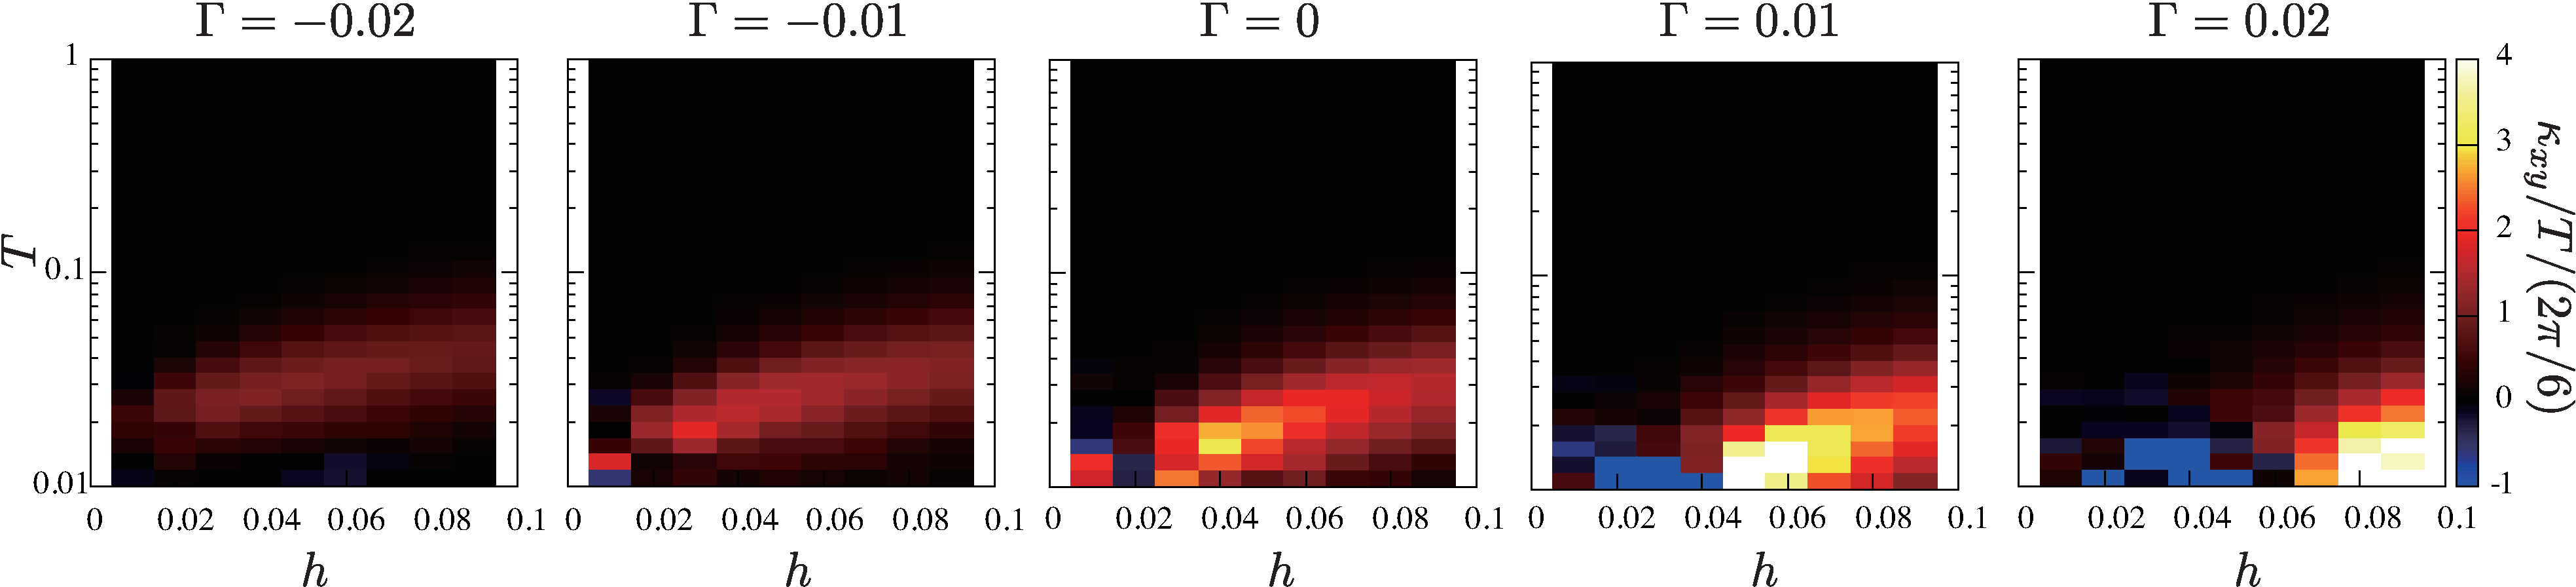
\includegraphics[width=\linewidth]{Figs/color_map_G.pdf}
  \end{center}
  \caption{Color maps of $\kappa_{xy}/T$ for ferromagnetic Kitaev model with $\Gamma = 0, \pm 0.01, \pm 0.02$ with various magnetic fields and temperatures.}
  \label{fig:color_map_G}
\end{figure*}

\begin{figure*}
  \begin{center}
    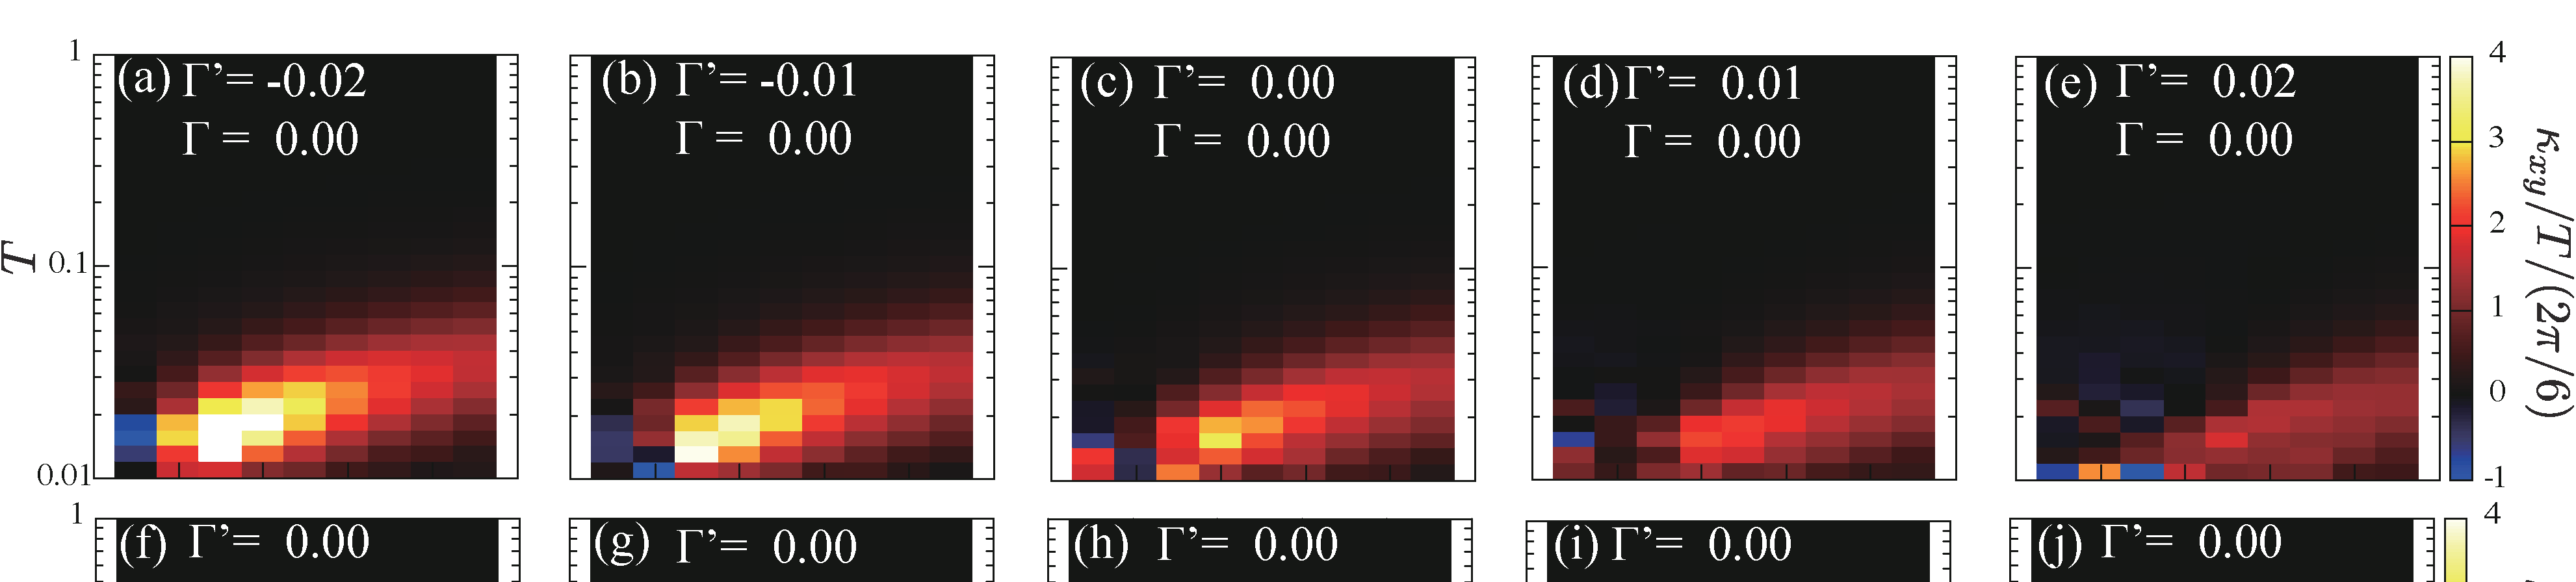
\includegraphics[width=\linewidth]{Figs/color_map_Gp.pdf}
  \end{center}
  \caption{Color maps of $\kappa_{xy}/T$ for ferromagnetic Kitaev model with $\Gamma' = 0, \pm 0.01, \pm 0.02$ with various magnetic fields and temperatures.}
  \label{fig:color_map_Gp}
\end{figure*}


\begin{figure*}
  \begin{center}
    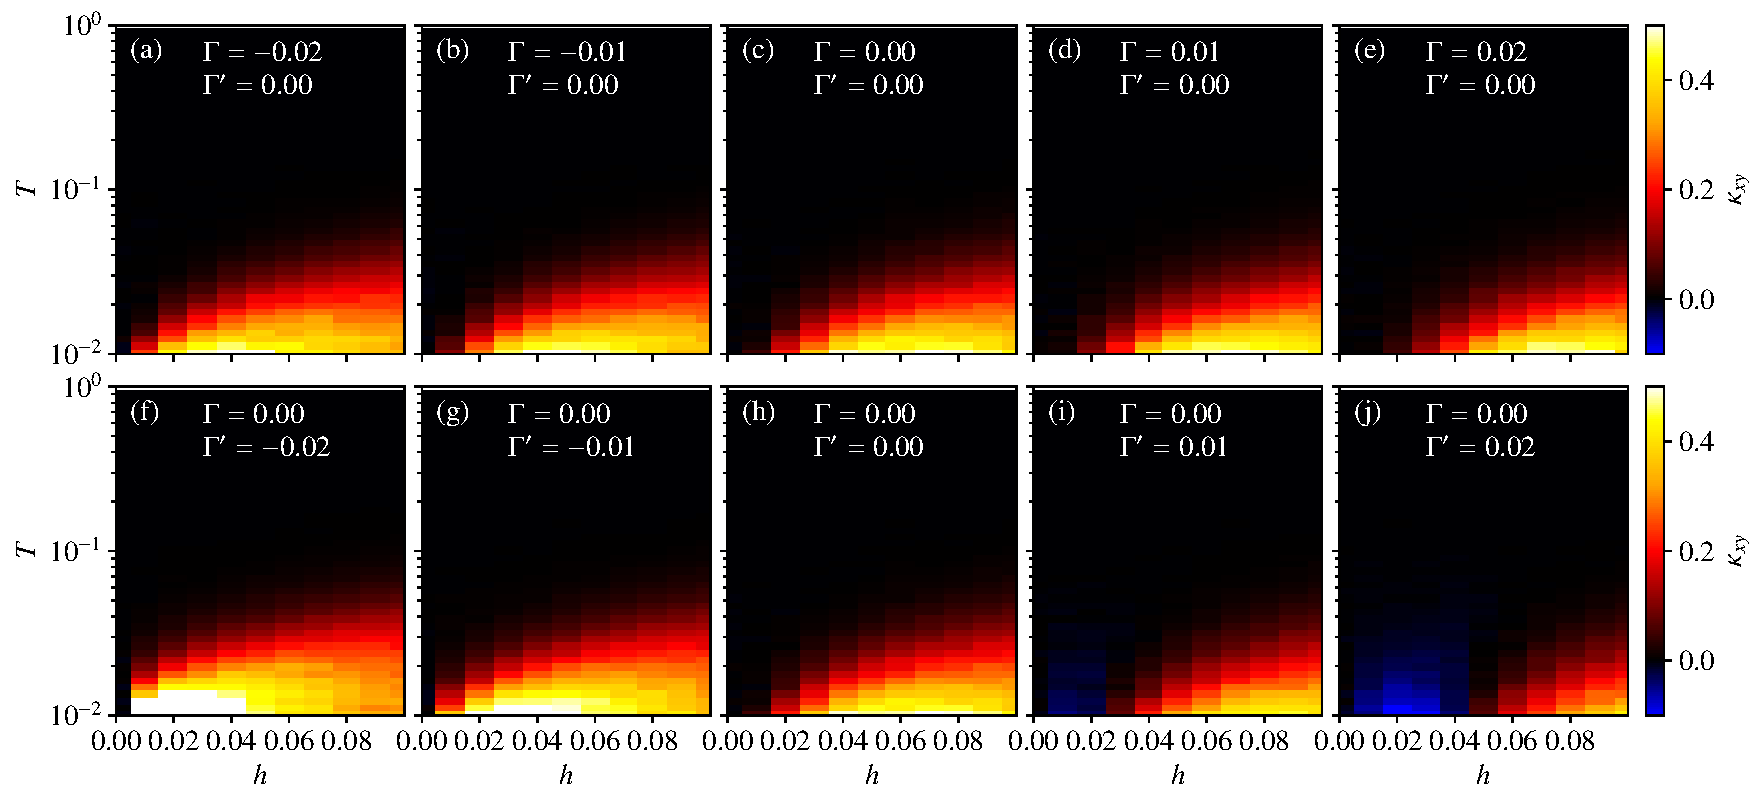
\includegraphics[width=\linewidth]{Figs/fig_cmap_classical.pdf}
  \end{center}
  \caption{\blue{Color maps of $\kappa_{xy}$ for the ferromagnetic Kitaev model with several values of $\Gamma$ and $\Gamma'$ on the plane of the magnetic field and temperature.}}
  \label{fig:cmap_classical}
\end{figure*}

  
\section{Summary}
In this study, ...


\appendix

\section{Benchmark on tensor network method}
\label{sec:XTRG_Bench}
In this section, we present several benchmark calculations for the tensor network method. 

Firstly, we show representative physical quantities of the pure Kitaev model on the $(L, L') = (6, 6)$ cylinder for bond-dimensions $D=300$, $400$, and $D=500$ in Fig.~\ref{fig:CMk_XC6}. Note, we showed the data for $D=500$. Although we see slightly larger $D$ dependencies for $T \lesssim 0.05$  for the specific heat and the thermal Hall conductivity in $h=0.04$, we obtained clear peak structures in $D=500$ and their values are not so deviated from those of $D=400$. Thus, we consider $D=500$ is sufficiently large to discuss the thermal Hall conductivity and related physics for $(L, L') = (6, 6)$.

In Fig.~\ref{fig:CMK_XC4}, we show the same physical quantities on the $(L, L') = (8, 4)$ cylinder for various bond-dimensions. In this geometry, up to $D=400$, we obtained almost converged data even for the specific heat and the thermal Hall conductivity at $h=0.04$. Note that the accuracy of the matrix product representation largely depends on the circumferenc


\begin{figure}
  \begin{center}
    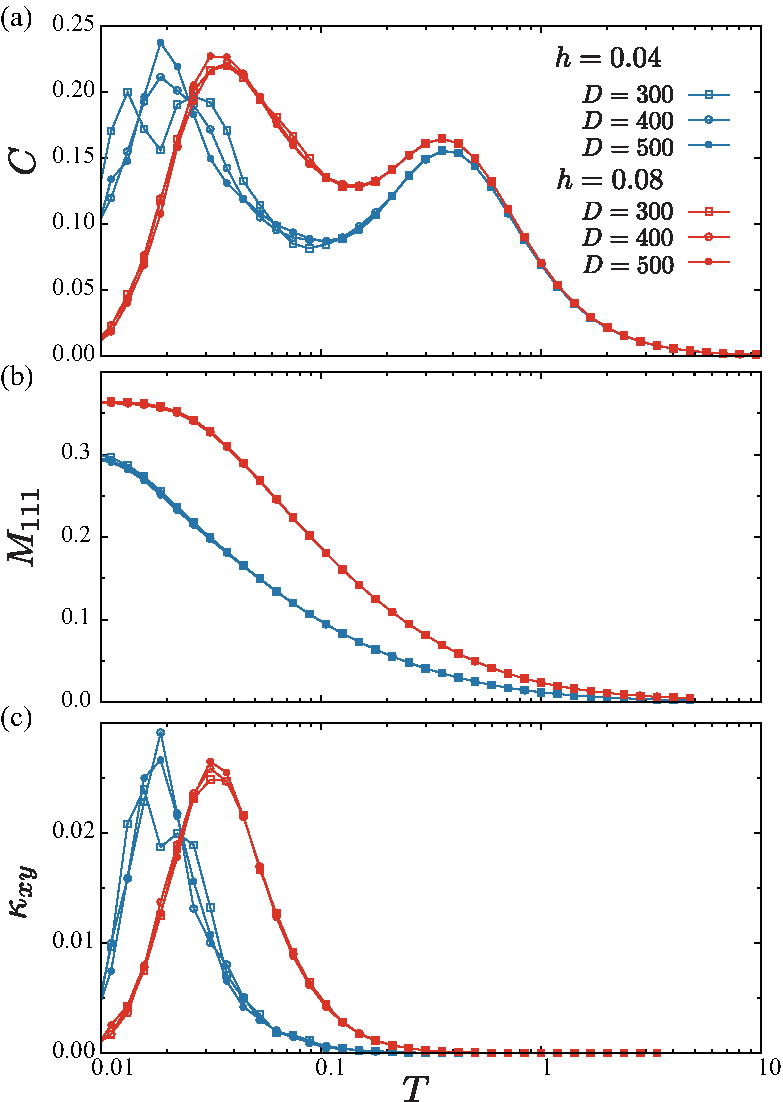
\includegraphics[width=0.9\linewidth]{Figs/plot_CMk.pdf}
  \end{center}
  \caption{Temperature dependence of (a) the specific heat (b) the magnetic moment, and (c) the thermal Hall conductivity of the ferromagnetic Kitaev model for the external magnetic field $h=0.04$ and $h=0.08$ parallel to $[111]$ direction with different bond-dimensions $D=300, 400, 500$. The lattice is \red{$(L, L') = (6, 6)$}}
  \label{fig:CMk_XC6}
\end{figure}
\begin{figure}
  \begin{center}
    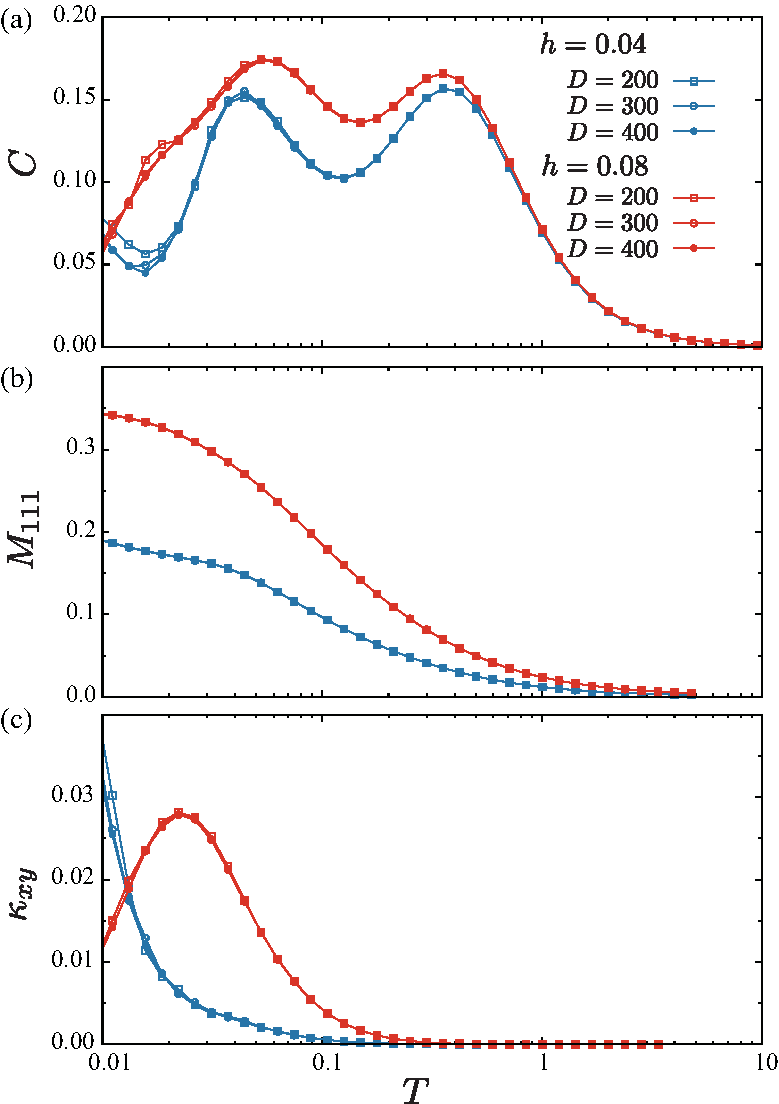
\includegraphics[width=0.9\linewidth]{Figs/plot_CMk_XC4.pdf}
  \end{center}
  \caption{Temperature dependence of (a) the specific heat (b) the magnetic moment, and (c) the thermal Hall conductivity of the ferromagnetic Kitaev model for the external magnetic field $h=0.04$ and $h=0.08$ parallel to $[111]$ direction with different bond-dimensions $D=200, 300, 400$. The lattice is \red{$(L, L') = (8, 4)$}.}
  \label{fig:CMk_XC4}
\end{figure}


\begin{figure}
  \begin{center}
    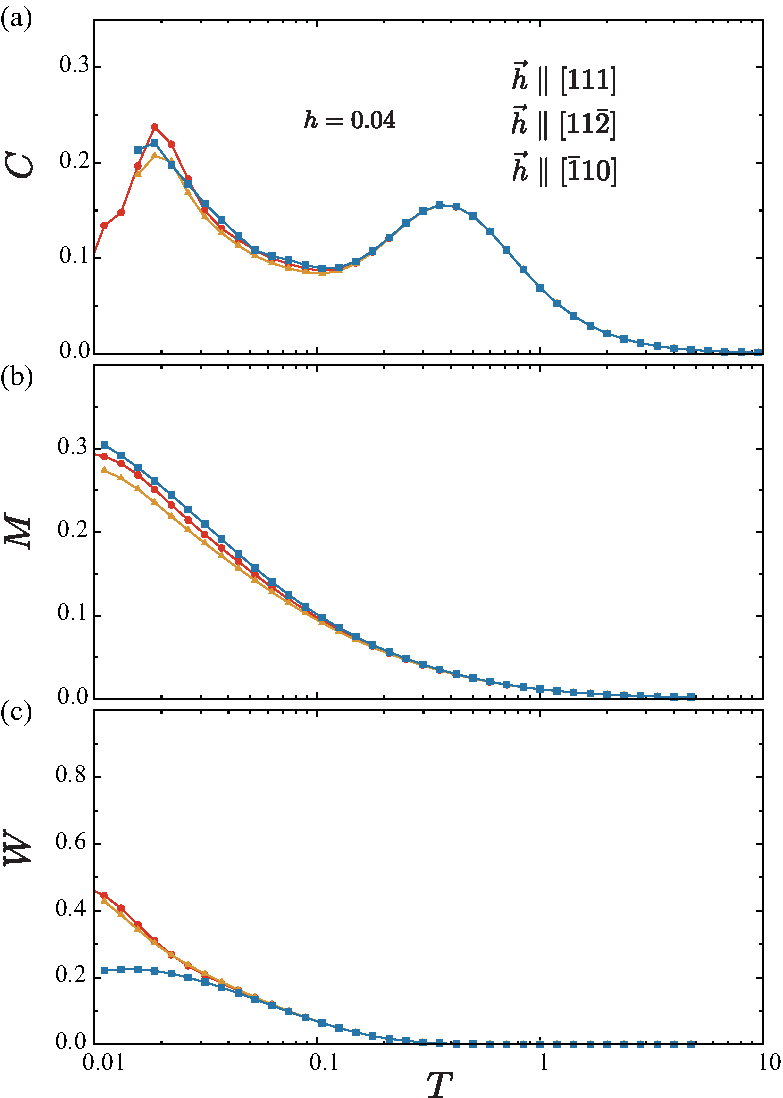
\includegraphics[width=0.9\linewidth]{Figs/plot_CMF_h0.04_ab.pdf}
  \end{center}
  \caption{Temperature dependence of (a) the specific heat (b) the magnetic moment, and (c) the flux of the ferromagnetic Kitaev model under magnetic fields parallel to $[111]$, $[11\bar{2}]$, and $[1\bar{1}0]$ with $|h|=0.04$.}
  \label{fig:CMF_h0.04_ab}
\end{figure}
\begin{figure}
  \begin{center}
    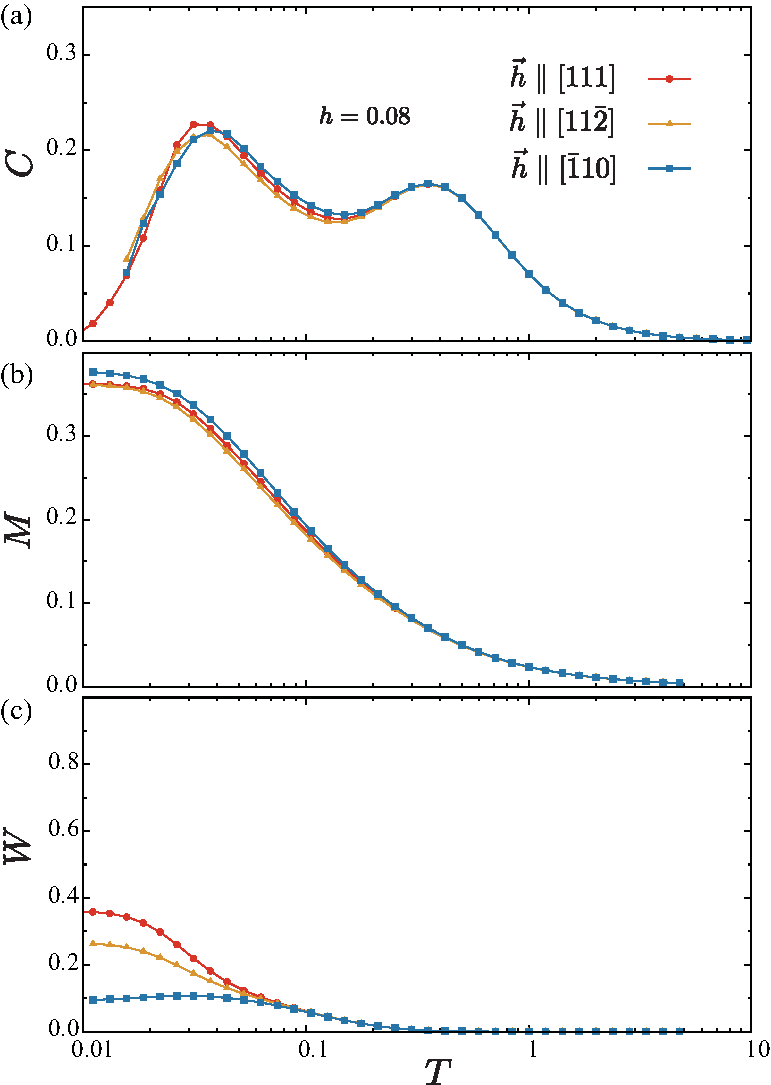
\includegraphics[width=0.9\linewidth]{Figs/plot_CMF_h0.08_ab.pdf}
  \end{center}
  \caption{Temperature dependence of (a) the specific heat (b) the magnetic moment, and (c) the flux of the ferromagnetic Kitaev model under magnetic fields parallel to $[111]$, $[11\bar{2}]$, and $[1\bar{1}0]$ with $|h|=0.08$.}
  \label{fig:CMF_h0.08_ab}
\end{figure}


\begin{figure*}
  \begin{center}
    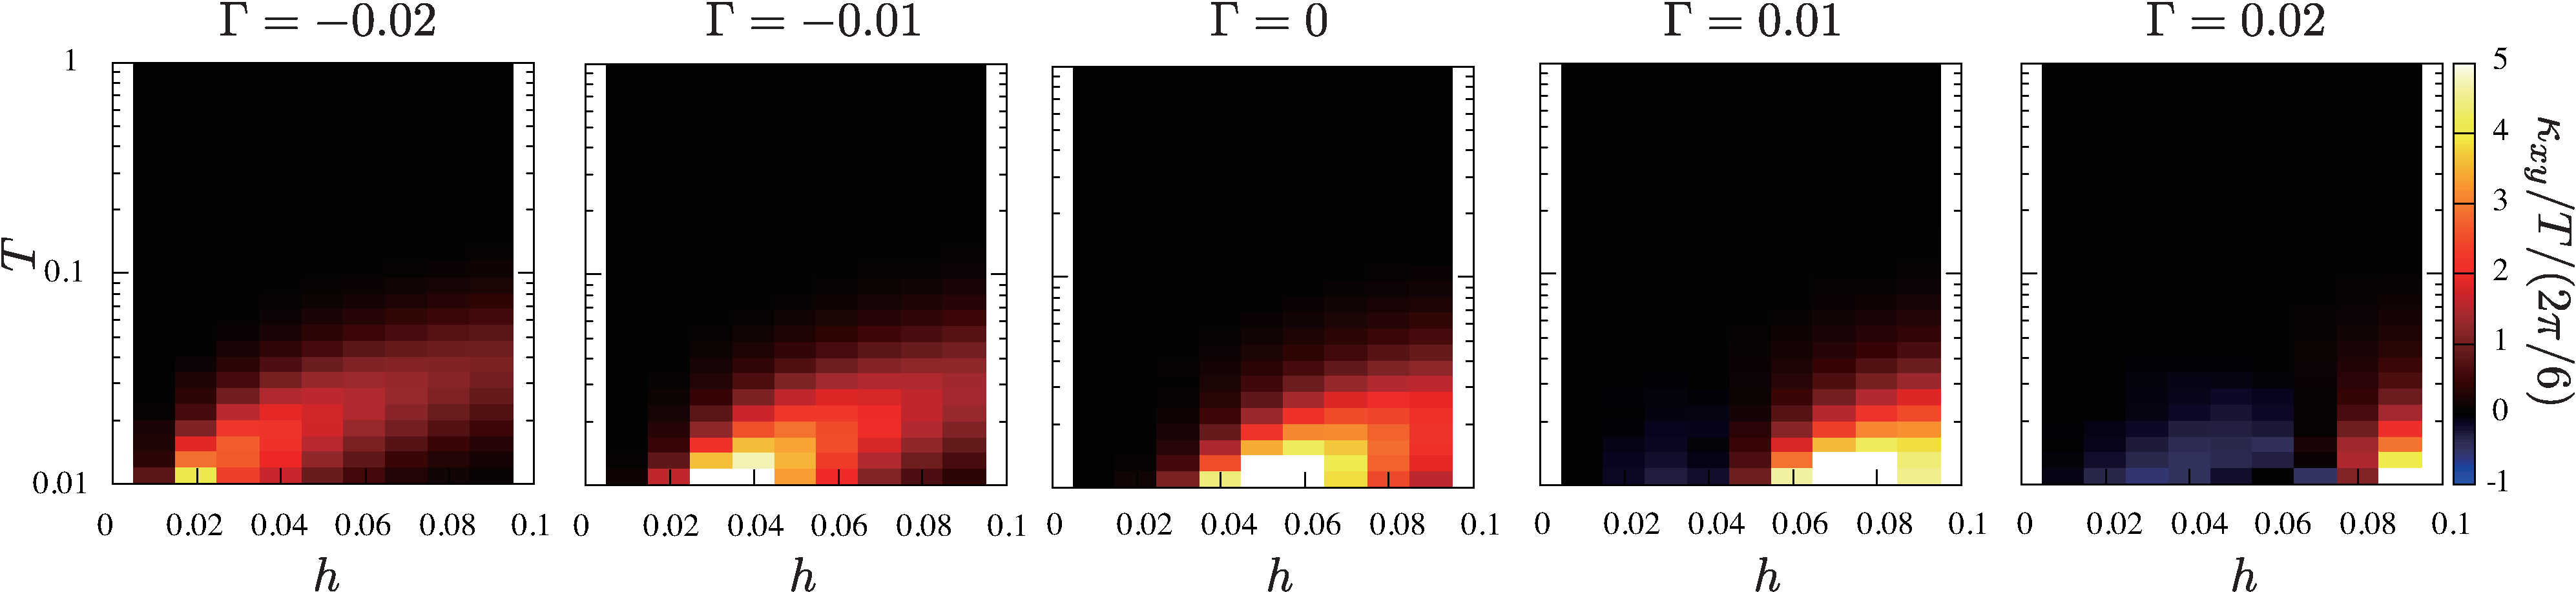
\includegraphics[width=\linewidth]{Figs/color_map_G_XC4.pdf}
  \end{center}
  \caption{Color maps of $\kappa_{xy}/T$ for ferromagnetic Kitaev model with $\Gamma = 0, \pm 0.01, \pm 0.02$ with various magnetic fields and temperatures. The lattice is \red{$(L, L') = (8, 4)$}.}
  \label{fig:color_map_G_XC4}
\end{figure*}

\begin{figure*}
  \begin{center}
    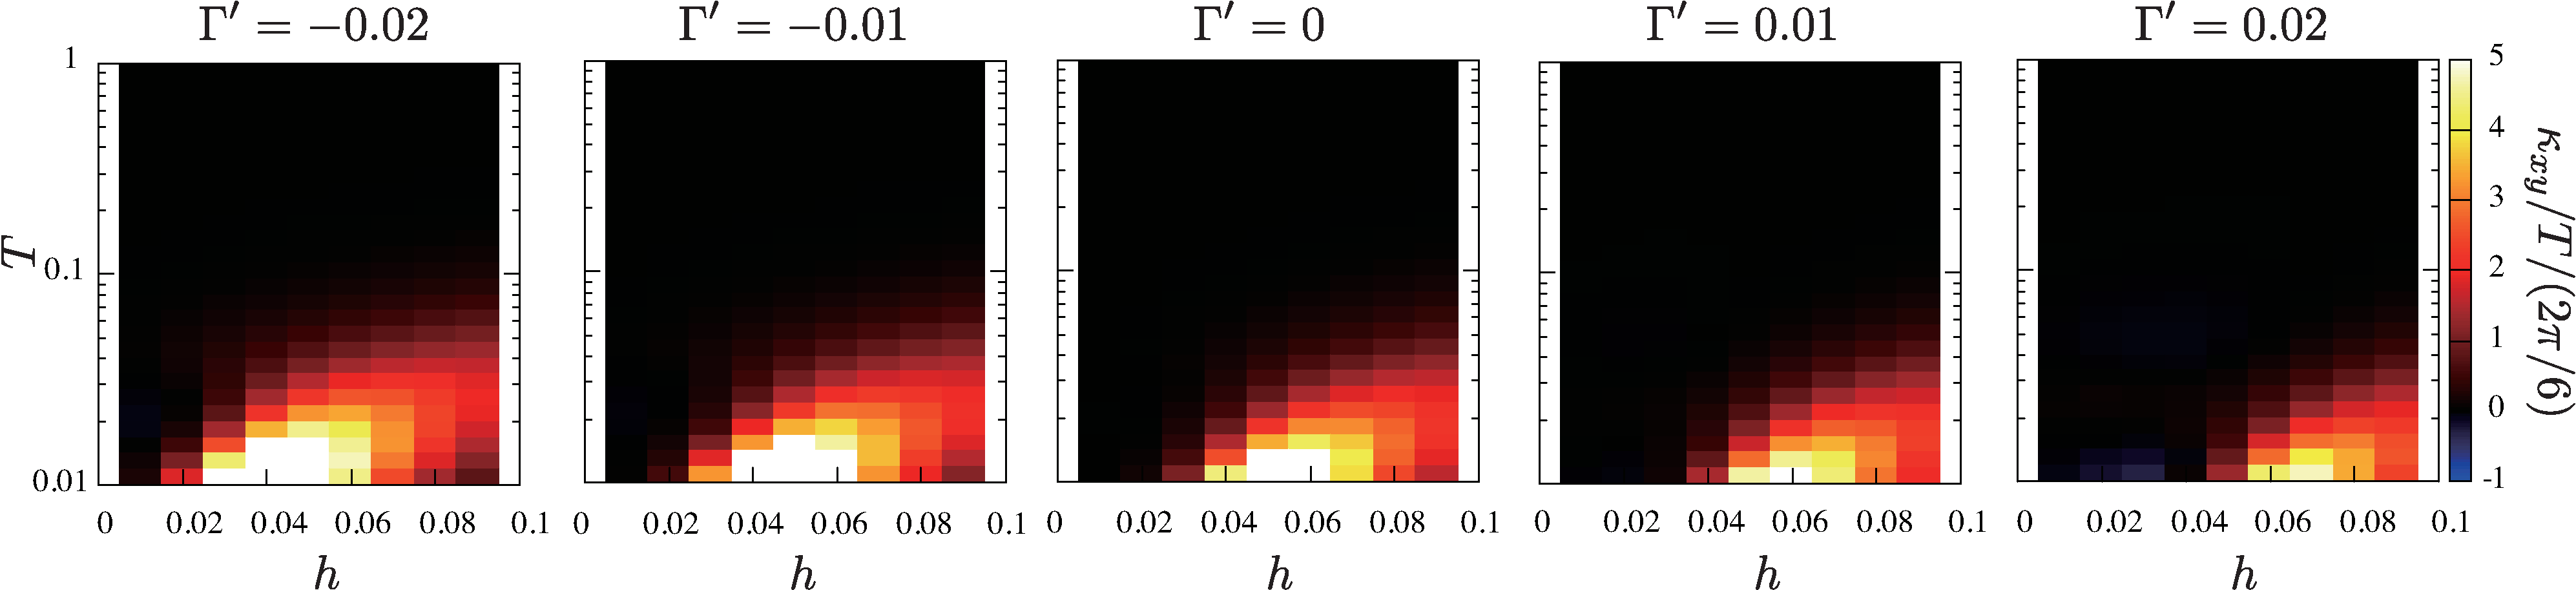
\includegraphics[width=\linewidth]{Figs/color_map_Gp_XC4.pdf}
  \end{center}
  \caption{Color maps of $\kappa_{xy}/T$ for ferromagnetic Kitaev model with $\Gamma' = 0, \pm 0.01, \pm 0.02$ with various magnetic fields and temperatures. The lattice is \red{$(L, L') = (8, 4)$}.}
  \label{fig:color_map_Gp_XC4}
\end{figure*}

\section{Benchmark on thermal pure quantum state}
We compare the results of the cTPQ method with
the full diagonalization for the \red{$(L, L') = (2, 4)$} cluster (the total system size is $N_{\rm s}=16$).
In the full exact diagonalization (full ED) method, we diagonalize Hamiltonian whose dimension is
$2^{16}=65536$ using ScaLAPACK~\cite{scalapack}. 
Using obtained eigenvalues and eigenvectors,
we calculate the temperature dependence of the physical quantities.

\if
% this part is not necessary
The definitions of the physical quantities are given as
\begin{align}
C&= \frac{\langle H^2\rangle-\langle H\rangle^2}{T^2}, \\
m&= (m_{x}^2+m_{y}^2+m_z^2)^{1/2}, \\
\kappa&= \frac{d J_{E}}{dT}, \\
J_{E} &= i[H,\vec{P}_{E}] \\ \notag
&=\sum_{[ijk]_{\gamma\gamma^{\prime}}}
\frac{\vec{r}_k-\vec{r}_i}{2}L_{ijk}^{\gamma\gamma^{\prime}}+
\sum_{\langle ij\rangle_{\gamma}}
\frac{\vec{r}_j-\vec{r}_i}{2}M_{ij}^{\gamma}, \\
L_{ijk}^{\gamma\gamma^{\prime}}&=\sum_{\alpha\beta\alpha^{\prime}\beta^{\prime}\gamma{\prime\prime}}
J_{\alpha\beta}^{\gamma}
J_{\alpha^{\prime}\beta^{\prime}}^{\gamma^{\prime}}
\epsilon_{\alpha\gamma^{\prime\prime}\alpha^{\prime}}
S_{i}^{\beta}S_{j}^{\gamma^{\prime\prime}}S_{k}^{\beta^{\prime}}, \\
M_{ij}^{\gamma}&= \sum_{\alpha\beta\gamma^{\prime}\gamma^{\prime\prime}}
J_{\alpha\beta}^{\gamma}h_{\gamma^{\prime}}\epsilon_{\gamma^{\prime}\alpha\gamma^{\prime\prime}}
(S_{i}^{\gamma^{\prime\prime}}S_{j}^{\beta}-S_{i}^{\beta}S_{j}^{\gamma^{\prime\prime}}).
\end{align}
\fi

At $|h|=0.04$, the specific heat $C$ has three-peak structures.
This three structure may be the finite-size effects 
since it vanishes for larger system sizes. %such as XC6L2.
Even at $|h|=0.08$, the hump in the specific heat 
still exists around $T=0.02$.
As shown in Fig.~\ref{comp_ED}(a),
the cTPQ method reproduces the temperature dependence 
of the specific heat for $|h|=0.04$ and $|h|=0.08$ including
the multiple peak structures.
Fig.~\ref{comp_ED}(b) shows 
the temperature dependence of the magnetization and
the cTPQ method also reproduces the results of the 
full exact diagonalization. 

\begin{figure}[t] 
\begin{center} 
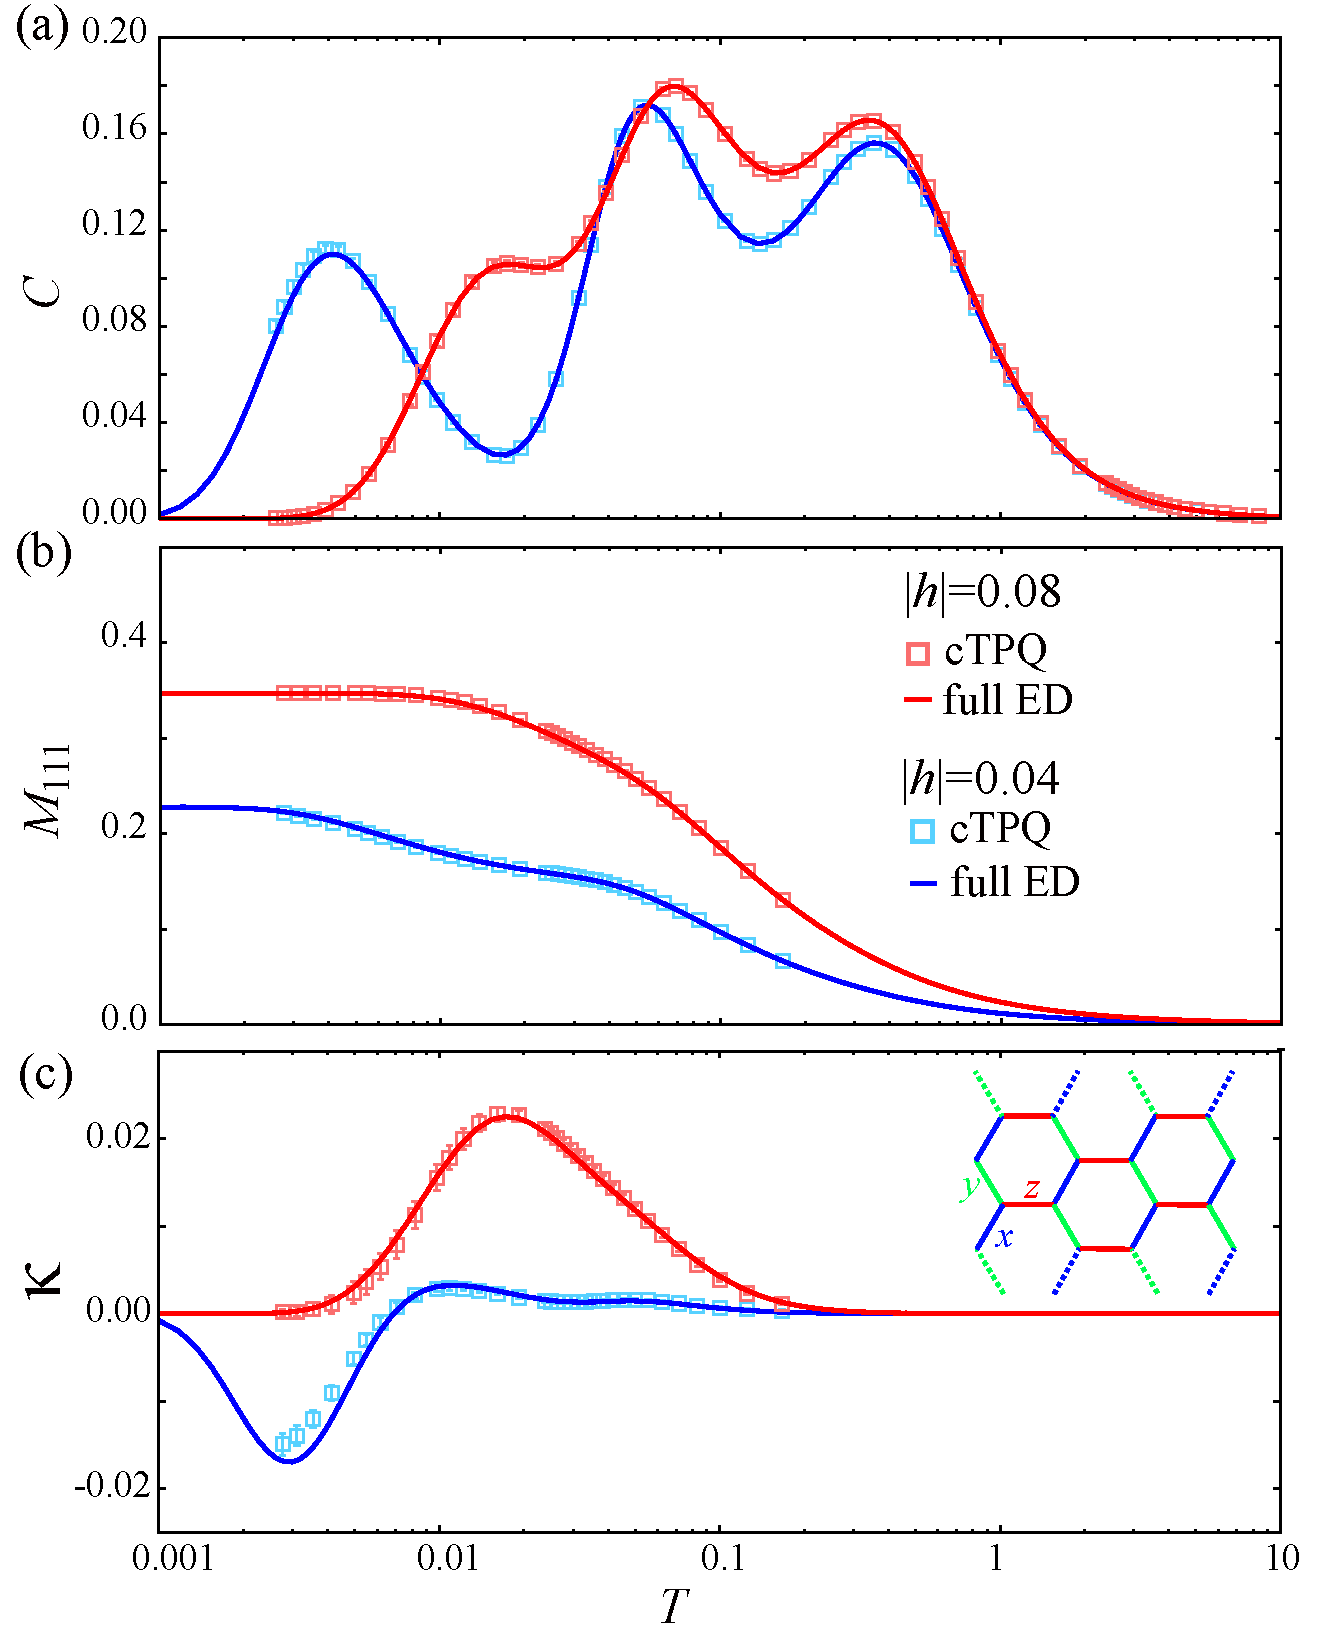
\includegraphics[width=0.9\linewidth]{Figs/compED_4_o.pdf}
\vspace{-0.5cm} 
\caption{Temperature dependence of (a) the specific heat, (b) the total magnetization, and
(c) the thermal Hall conductivity $\kappa$.
We take $N_{\rm tot}=P=1000,M=500$ in the bootstrap sampling.}
\label{comp_ED}
\end{center}
\end{figure}

We show the temperature dependence of the thermal 
Hall conductivity $\kappa$ in Fig.~\ref{comp_ED}(c).
The thermal Hall conductivity $\kappa$ at $|h|=0.04$
becomes negative below $T\leq 10^{-2}$. The negative $\kappa$ also may be 
caused by the finite size effects due to short length of the edges.
In fact, $\kappa$ becomes positive for larger system sizes as we show above.
The cTPQ method well reproduces this peculiar temperature 
dependence. At $h=0.08$, $\kappa$ shows 
a single peak structure and it is also well reproduced by the cTPQ method.
These consistencies with the results by the full ED demonstrate
the validity of the cTPQ method.
%\tr{{\bf for h=0.08, the agreement is not good. so, I now taking more samples.}}

\section{Comparison between tensor network method and thermal pure quantum state}
Here, we compare the results of the cTPQ method with those of the XTRG
for the \red{$(L, L') = (6, 2)$} cluster ($N_{\rm s}=24$). 
Fig.~\ref{comp_XTRG}(a) shows the temperature dependence of the specific heat. 
We find that both methods reproduce 
the two-peak structure in the specific heat, which is a 
characteristic feature in the Kitaev model. 
Except for the small discrepancy around the low-temperature peak 
at $|h|=0.04$, both independent methods agree well with each other
over the three magnitudes of the temperature scale.
This consistency demonstrates that the XTRG method gives the accurate results.
%Because the high-temperature peak corresponds to the energy scale of the
%formation of the itinerant Majorana fermions, it does
%not 

In Fig.~\ref{comp_XTRG}(b),
we show the temperature dependence of the magnetization.
In all the temperature regions, 
we find that both methods agree well within the error bars.
Since the magnetization is given by the first derivative of the
free energy, its fluctuation is expected to be small.
This may be the reason why the error bars of the magnetization
are smaller than those of the specific heat 
and the thermal Hall conductivity.

\magenta{We show the temperature dependence of $\kappa$
in Fig.~\ref{comp_XTRG}(c) and find that
$D=500$ already gives sufficiently accurate
results of the thermal Hall conductivity $\kappa$ except for the small deviations on the
peak values of $\kappa$. 
This result indicates that  
the XTRG calculations shown in this paper correctly capture the essence of the
thermal Hall conductivity in the extended Kitaev models.} 
%The XTRG method well reproduces the 

%temperature dependence of $\kappa$ obtained by the cTPQ method.
%Although the small deviations on the peak values of $\kappa$ 
%would vanish if we increase bond dimension $D$,
%the numerical cost becomes huge. 
%To perform the comprehensive calculations of the extended Kitaev models 
%in a wide range of the parameters, we take $D=500$ in the XTRG calculations.


\begin{figure}[tbh] 
\begin{center} 
%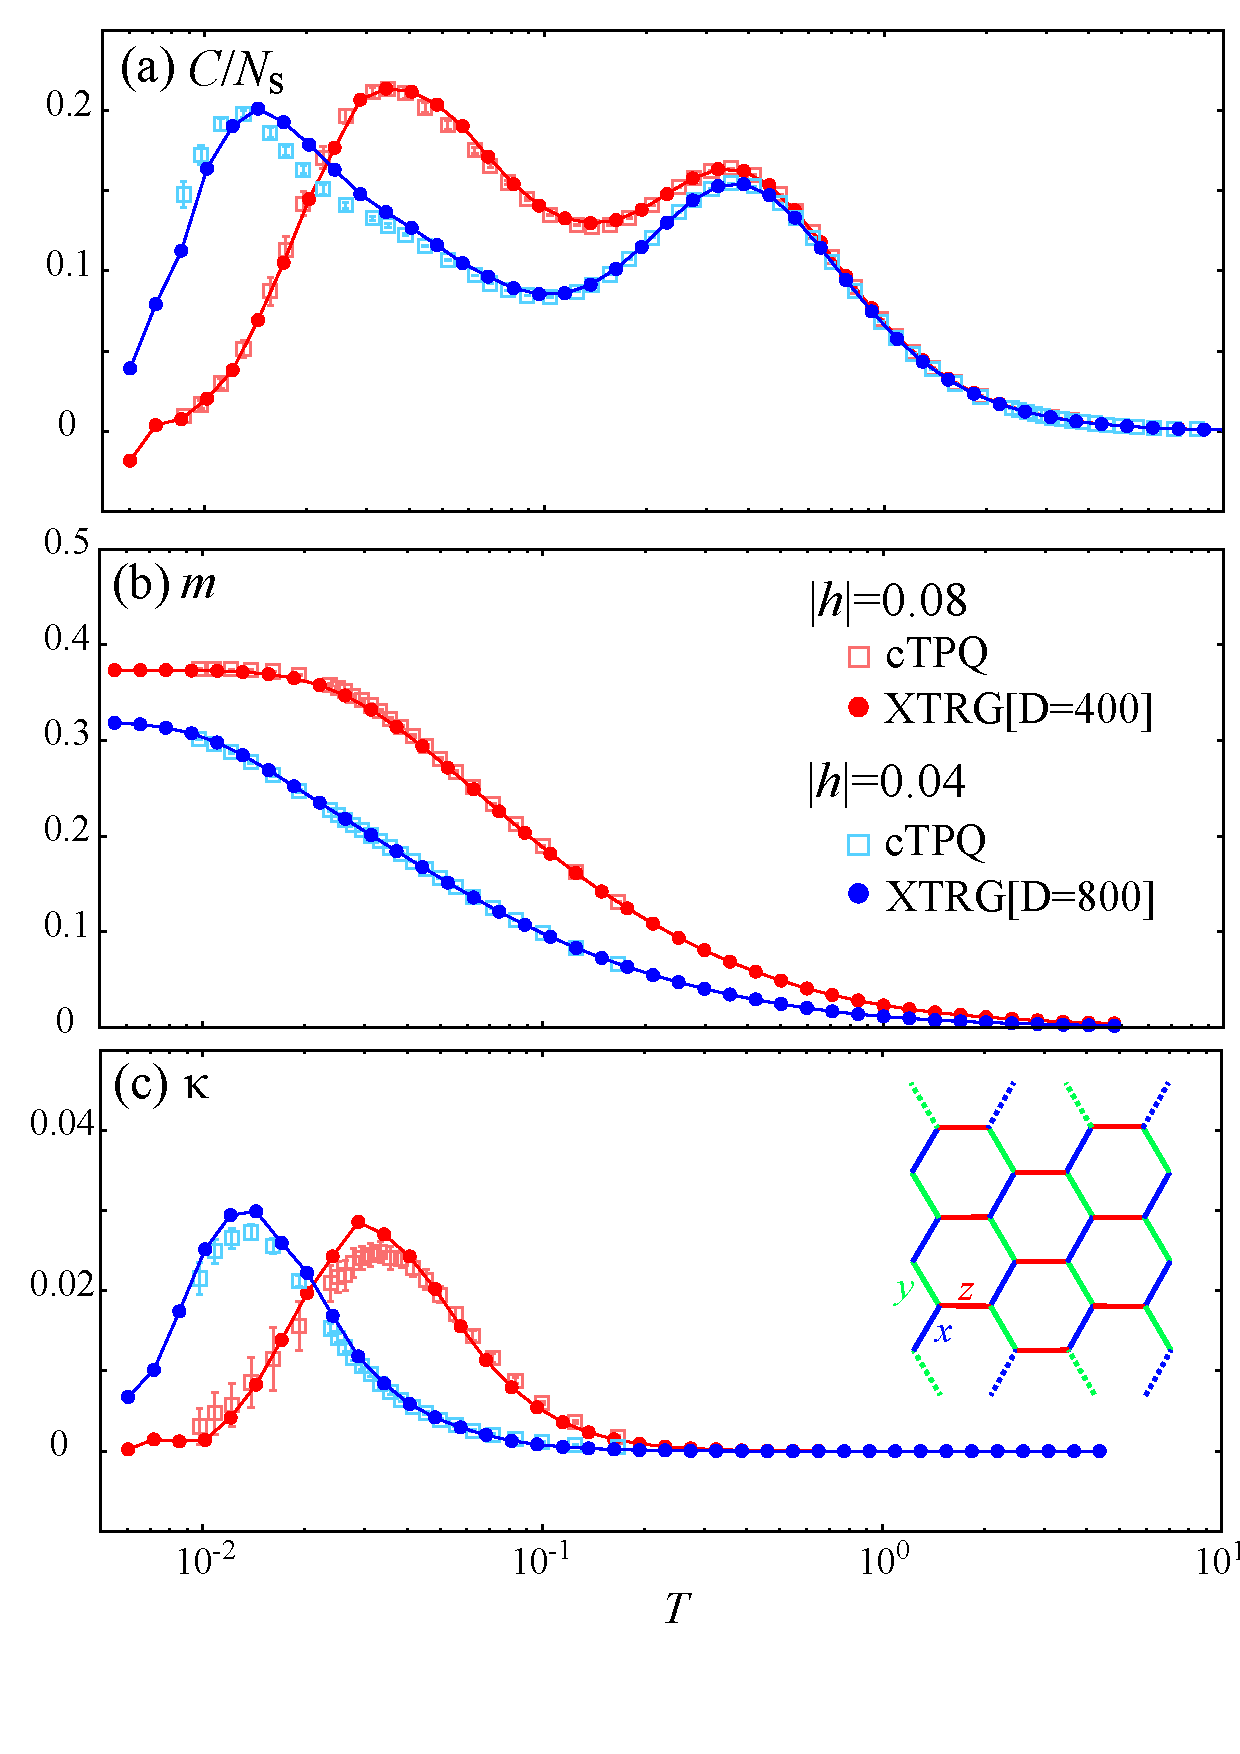
\includegraphics[width=0.9\linewidth]{comp_XTRG_o.pdf}
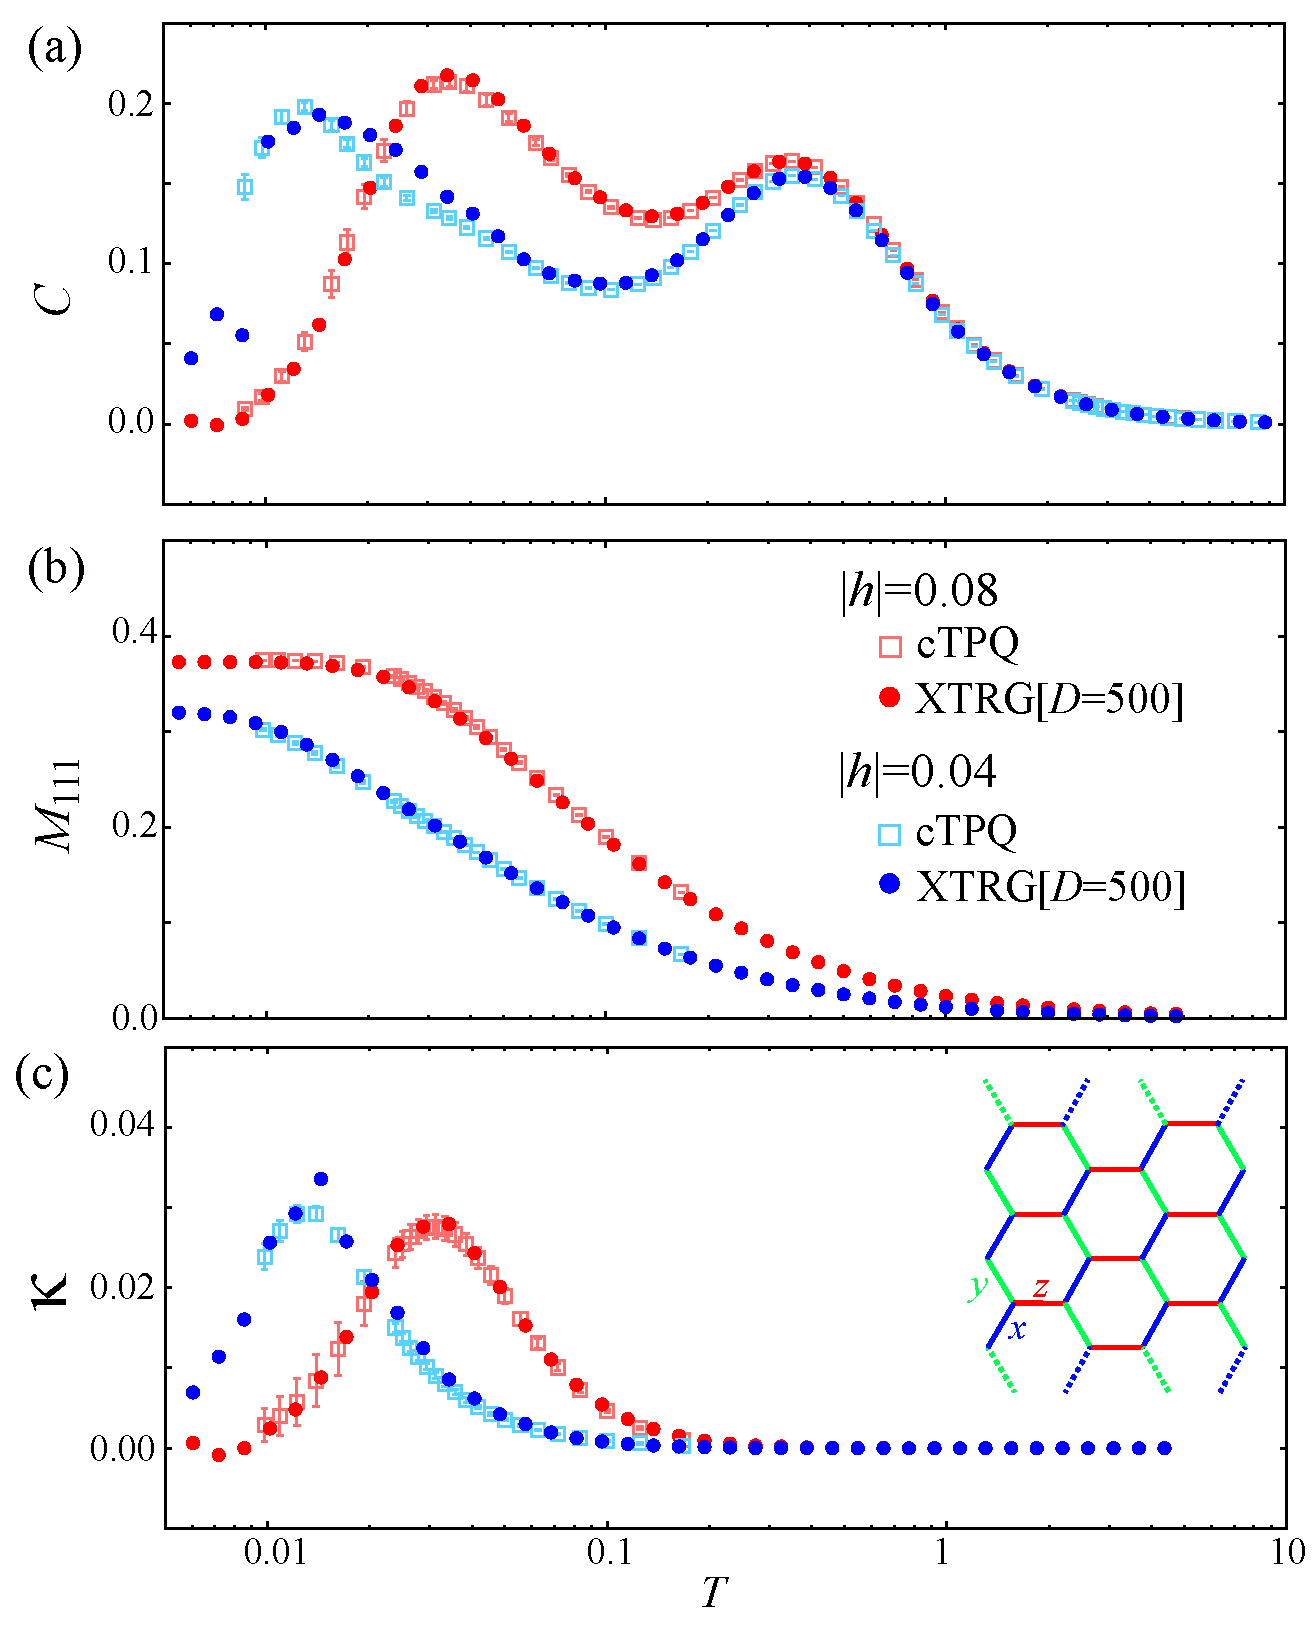
\includegraphics[width=0.9\linewidth]{Figs/compXTRG_3_o.pdf}
\vspace{-0.5cm} 
\caption{Temperature dependence of (a) the specific heat, (b) the total magnetization, and
(c) the thermal Hall conductivity $\kappa$. 
We take $N_{\rm tot}=P=100,M=50$ in the bootstrap sampling.}
\label{comp_XTRG}
\end{center}
\end{figure}

\bibliography{Kitaev_kxy}
\end{document}
